\documentclass[a4paper, 16pt]{article}
\usepackage[utf8]{inputenc}
\usepackage[english, russian]{babel} 
\usepackage[left=20mm, top=20mm, right=20mm,
 bottom=20mm, head=1mm, foot=1mm]{geometry}
\usepackage{tikz} 
\usepackage{amsmath, amsfonts, amssymb}
\usepackage{graphicx}
\usepackage{fancybox, fancyhdr}
\usepackage{hyperref}
\usepackage{listings}
\usepackage{caption}
\usepackage{subcaption}
\usepackage{xcolor}
\pagestyle{fancy}
\fancyhf{}
\fancyhead[L]{Лабораторная работа №5}
\fancyhead[R]{Техническое зрение}
\fancyfoot[C]{\thepage}
\graphicspath{{images/}}
\usetikzlibrary{patterns}
\definecolor{LightGray}{gray}{0.95}
\lstdefinestyle{pycode}{
    language=Python,
    basicstyle=\footnotesize\ttfamily,
    numbers=left,
    numberstyle=\tiny\color{gray},
    stepnumber=1,
    numbersep=5pt,
    backgroundcolor=\color{LightGray},
    showspaces=false,
    showstringspaces=false,
    showtabs=false,
    tabsize=4,
    captionpos=b,
    breaklines=true,
    breakatwhitespace=false,
    frame=single,
    rulecolor=\color{black},
    linewidth=\linewidth,
    keywordstyle=\color{red}\bfseries,
    commentstyle=\color{green!40!black},
    stringstyle=\color{purple},
    escapeinside={\%*}{*)},
    xleftmargin=0pt,
    framexleftmargin=0pt,
    framexrightmargin=0pt
}
\lstset{style=pycode}
\hypersetup{
    colorlinks=true,
    linkcolor=blue,
    filecolor=magenta,      
    urlcolor=cyan,
    pdftitle={contents setup},
    pdfpagemode=FullScreen,
}
\allowdisplaybreaks
\DeclareMathOperator{\sinc}{sinc}
\newcommand{\frc}[2]{\raisebox{2pt}{$#1$}\big/\raisebox{-3pt}{$#2$}}

\begin{document}
\begin{titlepage}

    \begin{center}
    \vfill
    
    Федеральное государственное автономное образовательное учреждение высшего образования\\
    «Национальный Исследовательский Университет ИТМО»\ \\
    
    \vfill
    {\large\bf ЛАБОРАТОРНАЯ РАБОТА №5\\
        ПО ПРЕДМЕТУ <<ТЕХНИЧЕСКОЕ ЗРЕНИЕ>>\\
        ПО ТЕМЕ <<ПРЕОБРАЗОВАНИЕ ХАФА>>}
    \vfill
        
    \begin{flushright}
        \begin{minipage}{.45\textwidth}
        {
            \hbox{Преподаватель:}
            \hbox{Шаветов C. В.}
            \hbox{}
            \hbox{Выполнили:} 
            \hbox{Румянцев А. А.}
            \hbox{Чебаненко Д. А.}
            \hbox{Овчинников П. А.}
            \hbox{}
            \hbox{Поток: ТЕХ. ЗРЕНИЕ 2.1}
            \hbox{Факультет: СУиР}
            \hbox{Группа: R3241}
        }
        \end{minipage}
    \end{flushright}
    
    \vfill
            
    Санкт-Петербург\\
    2024
    \end{center}
    \end{titlepage}
    \setlength{\parskip}{1.5mm}
    
    \tableofcontents

    \newpage
    \setlength{\headheight}{12pt}
    \setlength{\footskip}{12pt}


    \section{Цель работы}
    \noindent Освоение преобразования для поиска геометрических примитивов.

    
    \section{Теоретическое обоснование применяемого преобразования для поиска геометрических примитивов}
    \noindent Идея преобразования Хафа заключается в поиске общих геометрических точек (ГМТ).
    
    
    \noindent Данный подход может использоваться для построения треугольника по трем заданным сторонам. 
    Сначала откладывается одна сторона треугольника, после этого концы отрезка рассматриваются как центры
    окружностей радиусами равными длинам второго и третьего отрезков. Место пересечения двух окружностей
    является общим ГМТ, откуда проводятся отрезки до концов первого отрезка. Другими словами, было проведено
    \textit{голосование} двух точек в пользу вероятного расположения третьей веришны треугольника.
    В результате <<голосования>> <<победила>> точка, набравшая два голоса. Ниже приведен соответствующий
    рисунок \ref{Рис:1}.
    \begin{figure}[!htb]
        \centering
        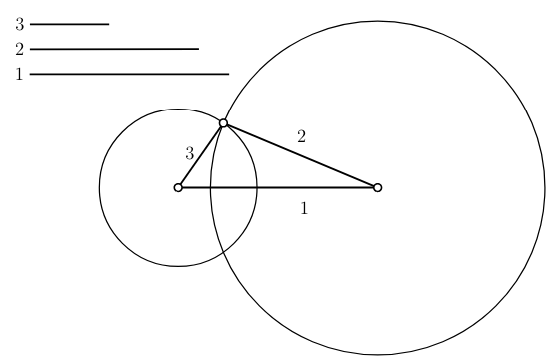
\includegraphics[scale=1]{triang.png}
        \captionsetup{skip=0pt}
        \caption{Построение треугольника по трем заданным сторонам.}
        \label{Рис:1}
    \end{figure}


    \noindent Для работы с реальными данными обобщим данную идею, чтобы работать с б\'{о}льшим количеством
    характерестических точек на изображении, участвующих в голосовании. Допустим, необходимо найти в бинарном
    точечном множестве окружность известного радиуса $R$, причем в данном множестве могут присутствовать и ложные 
    точки, не лежащие на искомой окружности. Набор центров возможных окружностей искомого радиуса вокруг каждой
    характеристической точки образует окружность радиуса $R$. Тогда, точка, соответствующая максимальному
    пересечению числа окружностей, и будет являться центром окружности искомого радиуса. Ниже приведен соответствующий
    рисунок \ref{Рис:2}.
    \begin{figure}[!htb]
        \centering
        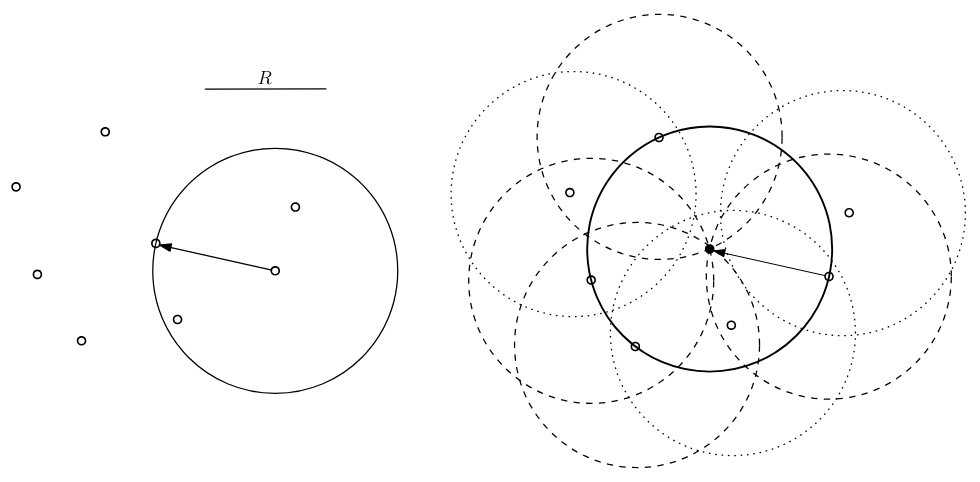
\includegraphics[scale=0.75]{circs.png}
        \captionsetup{skip=0pt}
        \caption{Обнаружение окружности известного радиуса в точечном множестве.}
        \label{Рис:2}
    \end{figure}


    \noindent В данной лабораторной работе используется классическое преобразование Хафа, базирующееся на
    рассмотренной идее голосования точек. Преобразование изначально было предназначено для выделения прямых
    на бинарных изображениях. В преобразовании Хафа для поиска геометрических примитивов используется пространство
    параметров. Самое распространенное параметрическое уравнение прямых приведено ниже.
    \begin{align}
        & y=kx+b,\label{eq:one}\\
        & x\cos{\theta}+y\sin{\theta}=\rho,\label{eq:two}
    \end{align}
    где $\rho$ -- радиус-вектор, проведенный из начала координат до прямой; $\theta$ -- угол наклона радиус-вектора.


    \noindent Пусть в декартовой системе координат прямая задана уравнением \eqref{eq:one}, из которого легко вычислить
    радиус-вектор $\rho$ и угол $\theta$ \eqref{eq:two}. Тогда в пространстве параметров Хафа прямая будет представлена
    точкой с координатами $(\rho_0,\theta_0)$. Ниже представлен соответствующий рисунок \ref{Рис:3}.
    \begin{figure}[!htb]
        \centering
        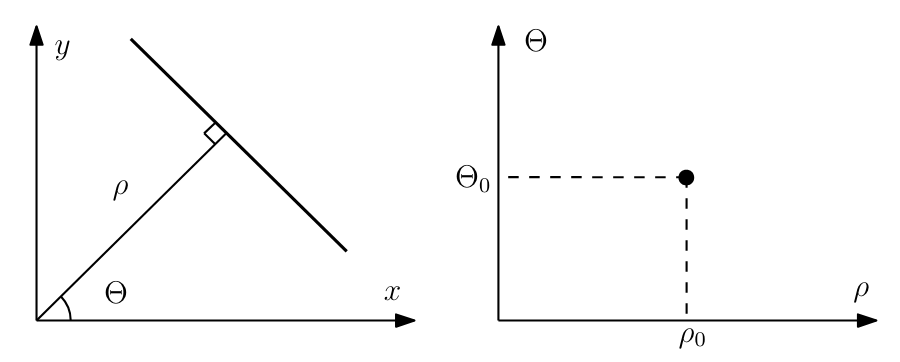
\includegraphics[scale=0.8]{line.png}
        \captionsetup{skip=0pt}
        \caption{Представление прямой в пространстве Хафа.}
        \label{Рис:3}
    \end{figure}


    \noindent Подход преобразования Хафа заключается в суммировании для каждой точки пространства количества поданных за нее голосов.
    Вследствие этого в дискретном виде пространство Хафа называется \textit{аккумулятором} и представляет собой некую матрицу
    $A(\rho,\theta)$, хранящую информацию о голосовании. В декартовой системе координат через каждую точку можно провести бесконечное
    число прямых. Их совокупность породит в пространстве параметров синусоидальную функцию отклика. Таким образом, любые две синусоидальные
    функции отклика в пространстве параметров пересекутся в точке $(\rho,\theta)$, только если порождающие их точки в исходном пространстве
    лежат на прямой. Выходит, что для поиска прямых в исходном пространстве необходимо найти все локальные максимумы аккумулятора. Ниже
    представлен соответствующий рисунок \ref{Рис:4}.
    \begin{figure}[!htb]
        \centering
        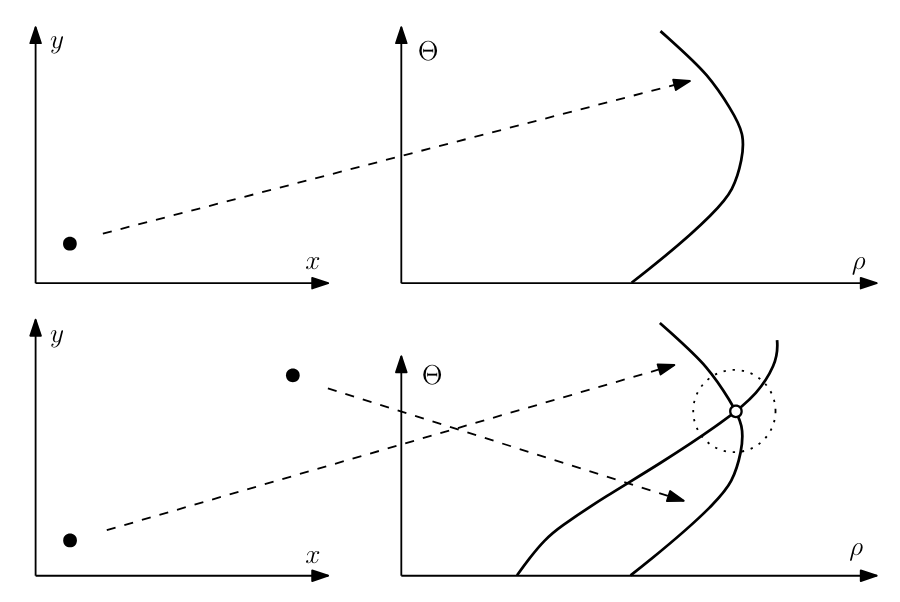
\includegraphics[scale=0.8]{voices.png}
        \captionsetup{skip=0pt}
        \caption{Процедура голосования.}
        \label{Рис:4}
    \end{figure}


    \noindent Рассмотренный алгоритм является универсальным. Его можно использовать для поиска любой другой кривой, описываемой в пространстве
    некоторой функцией с определенным числом параметров $F=(a_1,a_2,\hdots ,a_n,x,y)$, что повлияет только на размерность пространства параметров.


    \noindent Воспользуемся преобразованием Хафа для поиска окружностей заданного радиуса $R$. Окружность на плоскости описывается формулой
    $(x-x_0)^2+(y-y_0)^2=R^2$. Набор центров всех возможных окружностей радиуса $R$, проходящих через характеристическую точку, образует
    окружность радиуса $R$ вокруг этой точки. Вследствие этого функция отклика в преобразовании Хафа для поиска окружностей представляет
    окружность такого же размера с центром в голосующей точке. Таким образом, аналогично предыдущему случаю необходимо найти локальные
    максимумы аккумуляторной функции $A(x,y)$ в пространстве параметров $(x,y)$, которые и будут являться центрами искомых окружностей.


    \noindent Преобразование Хафа позволяет обнаруживать линии инвариантно не только к аффинным преобразованиям плоскости, но и к группе
    проективных преобразований в пространстве, так как преобразование инвариантно к сдвигу, масштабированию и повороту, при этом при проективных
    преобразованиях трехмерного пространства прямые линии всегда переходят только в прямые линии (в вырожденном случае -- в точки).


    \section{Ход выполнения работы}
    \subsection{Поиск прямых}
    \noindent Выберем три произвольных изображения, содержащих прямые.
    \begin{figure}[htbp]
        \centering
        \begin{subfigure}{0.3\textwidth}
            \centering
            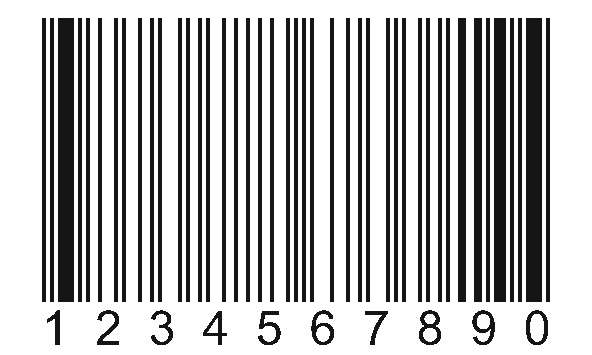
\includegraphics[width=\linewidth]{i1.png}
            \caption{Штрихкод}
            \label{fig:i1}
        \end{subfigure}
        \hfill
        \begin{subfigure}{0.3\textwidth}
            \centering
            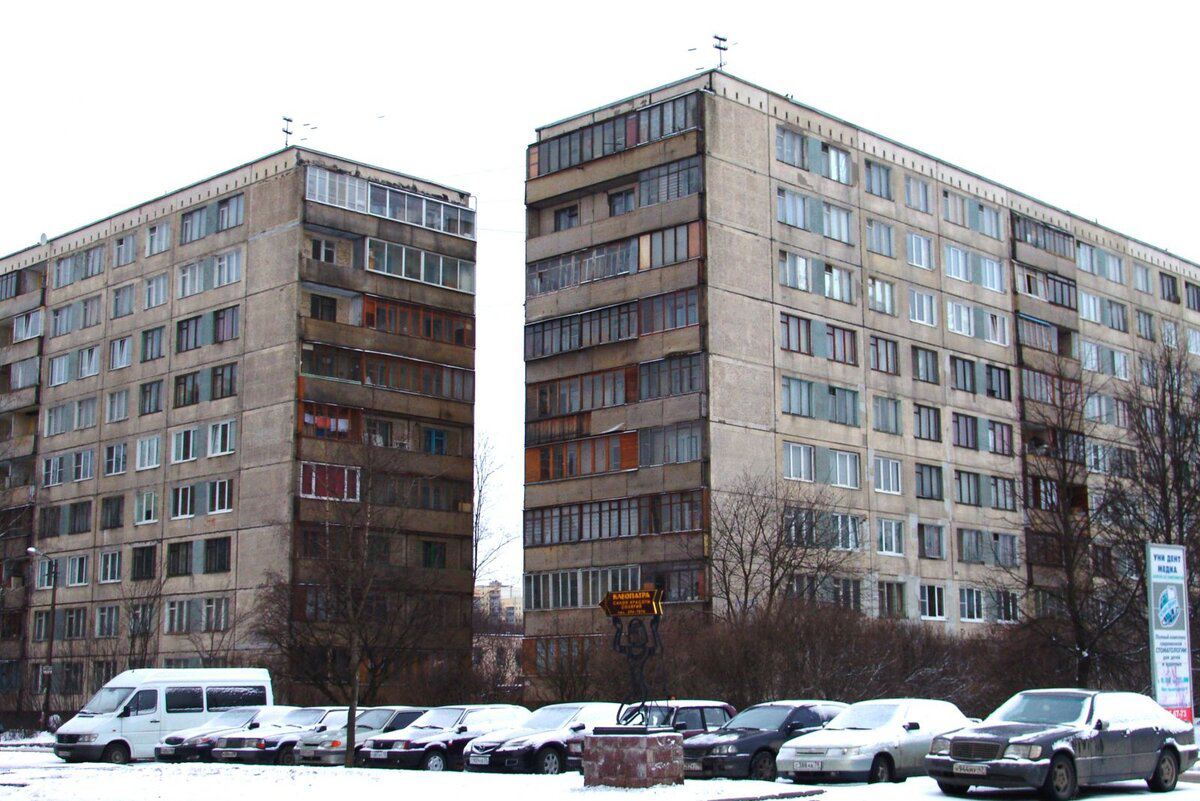
\includegraphics[width=\linewidth]{i2.png}
            \caption{Архитектура}
            \label{fig:i2}
        \end{subfigure}
        \hfill
        \begin{subfigure}{0.3\textwidth}
            \centering
            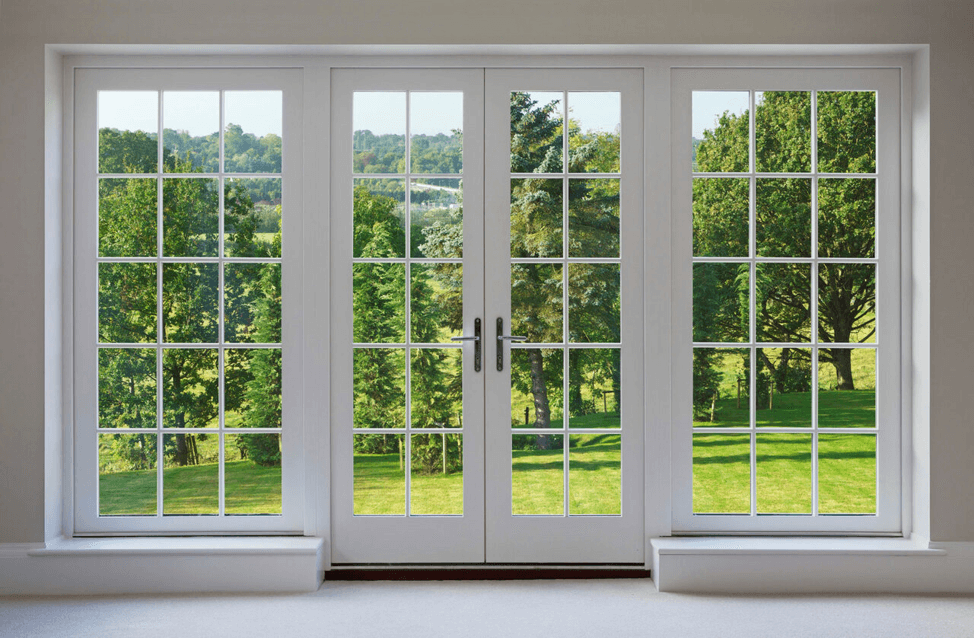
\includegraphics[width=\linewidth]{i3.png}
            \caption{Интерьер}
            \label{fig:i3}
        \end{subfigure}
        \caption{Произвольные изображения, содержащие прямые.}
        \label{fig:is}
    \end{figure}


    \noindent Попробуем сразу применить преобразование Хафа без использования каких-либо дифференциальных операторов.
    Сначала преобразуем изображение к оттенкам серого, далее применим Хафа и нарисуем линии на оригинальном изображении.
    \begin{figure}[htbp]
        \centering
        \begin{subfigure}{0.3\textwidth}
            \centering
            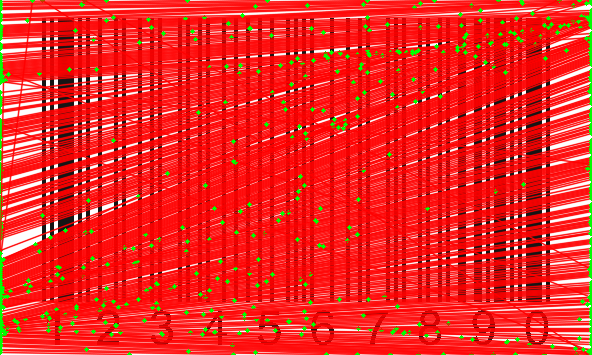
\includegraphics[width=\linewidth]{hl_i1.png}
            \caption{Штрихкод}
            \label{fig:hl_i1}
        \end{subfigure}
        \hfill
        \begin{subfigure}{0.3\textwidth}
            \centering
            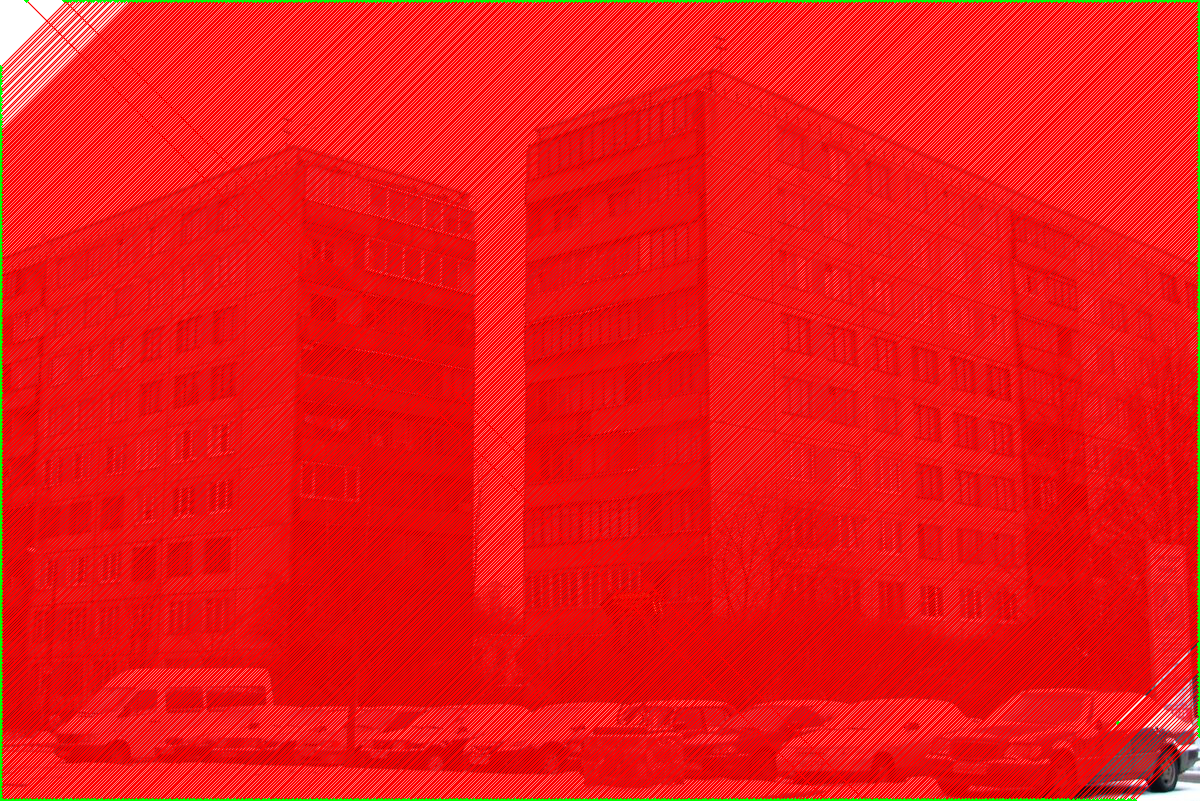
\includegraphics[width=\linewidth]{hl_i2.png}
            \caption{Архитектура}
            \label{fig:hl_i2}
        \end{subfigure}
        \hfill
        \begin{subfigure}{0.3\textwidth}
            \centering
            
\includegraphics[width=\linewidth]{hl_i3.png}
            \caption{Интерьер}
            \label{fig:hl_i3}
        \end{subfigure}
        \caption{Преобразование Хафа на выбранных изображениях.}
        \label{fig:hl_is}
    \end{figure}


    \noindent Исходя из результатов сделан вывод, что рассматривать преобразование Хафа без какой-либо
    подготовки изображения не нужно, так как линии вышли хаотичными и не соответствуют ожиданиям. Их
    исследование не внесет пользы в общий результат выполнения работы. Предположительно, шум, не достаточно
    четкие границы объектов и небинарное представление картинки привели к соответствующим изображениям.


    \newpage
    \noindent Обработаем изображения алгоритмом Кэнни -- оператором обнаружения границ изображения. Основными
    этапами алгоритма являются сглаживание изображения (для удаления шума), поиск градиентов (границы отмечаются там,
    где градиент изображения приобретает максимальное значение), подавление немаксимумов (только локальные максимумы
    отмечаются как границы), двойная пороговая фильтрация (потенциальные границы определяются порогами) и трассировка
    области неоднозначности (итоговые границы определяются путём подавления всех краёв, не связанных с определенными
    (сильными) границами). Перед обработкой изображение было преобразовано в оттенки серого, чтобы уменьшить вычислительные затраты.
    \begin{figure}[htbp]
        \centering
        \begin{subfigure}{0.3\textwidth}
            \centering
            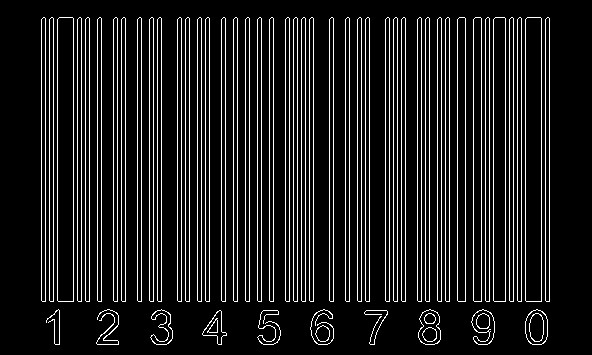
\includegraphics[width=\linewidth]{canny_i1.png}
            \caption{Штрихкод}
            \label{fig:canny_i1}
        \end{subfigure}
        \hfill
        \begin{subfigure}{0.3\textwidth}
            \centering
            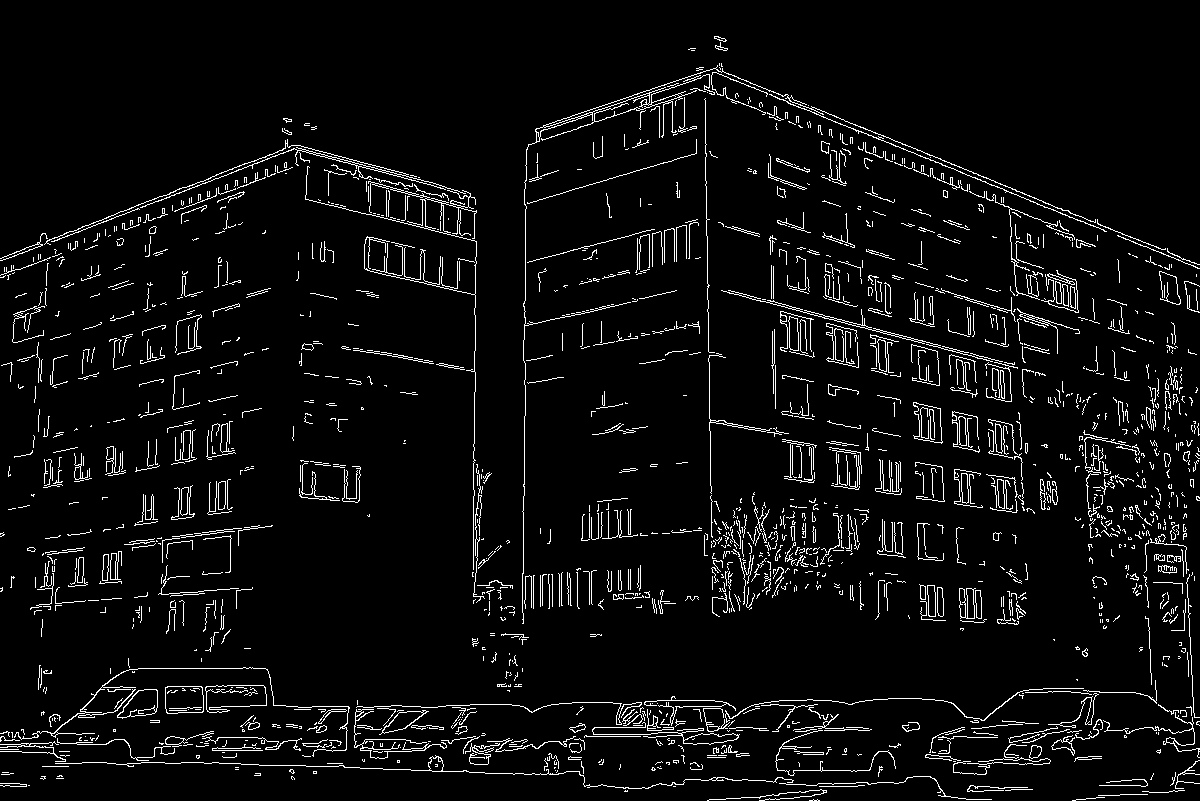
\includegraphics[width=\linewidth]{canny_i2.png}
            \caption{Архитектура}
            \label{fig:canny_i2}
        \end{subfigure}
        \hfill
        \begin{subfigure}{0.3\textwidth}
            \centering
            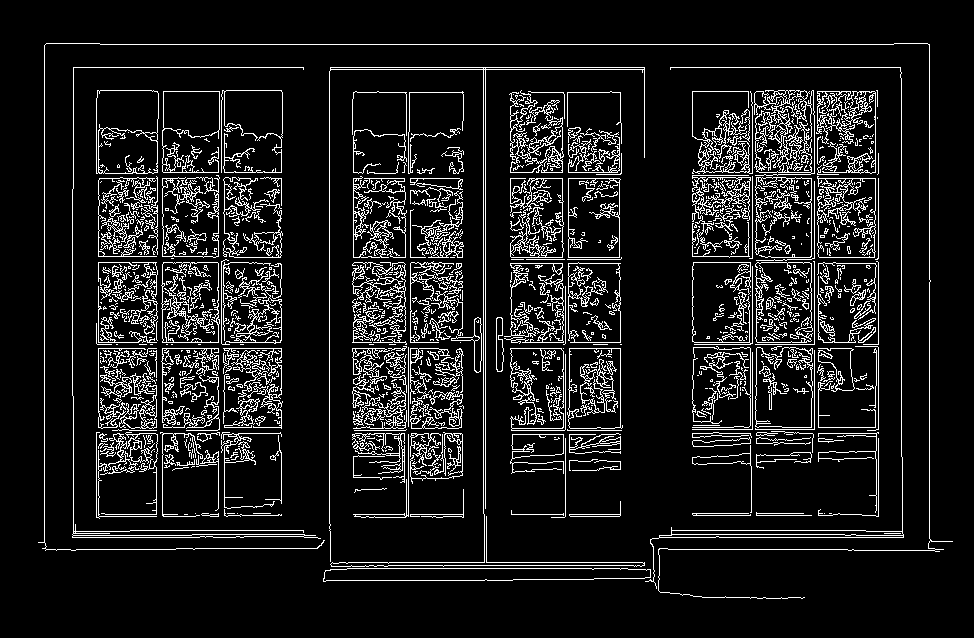
\includegraphics[width=\linewidth]{canny_i3.png}
            \caption{Интерьер}
            \label{fig:canny_i3}
        \end{subfigure}
        \caption{Алгоритм Кэнни на выбранных изображениях.}
        \label{fig:canny_is}
    \end{figure}


    \noindent Преобразуем изображения алгоритмом Хафа и получим результат, представленный на рисунке \ref{fig:canny_hl_is}.
    Найденные линии отрисованы красным цветом, точки начала и конца каждой линии отмечены зеленым цветом.
    Ниже каждой картинки написаны длина в пикселях самой длинной и самой короткой линий, а также количество отрисованных линий.
    \begin{figure}[htbp]
        \centering
        \begin{subfigure}{0.3\textwidth}
            \centering
            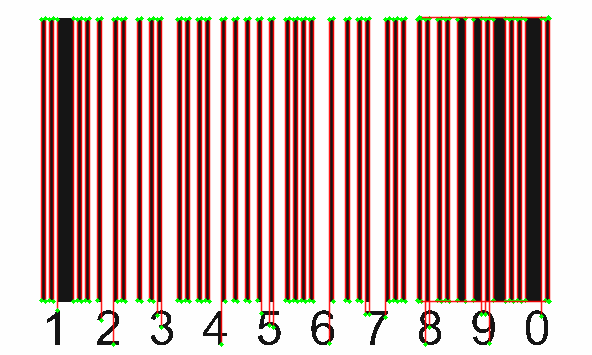
\includegraphics[width=\linewidth]{canny_hl_i1.png}
            \caption{Штрихкод\\Максимальная длина линии: 325p\\Минимальная длина линии: 129p\\Всего линий: 88}
            \label{fig:canny_hl_i1}
        \end{subfigure}
        \hfill
        \begin{subfigure}{0.3\textwidth}
            \centering
            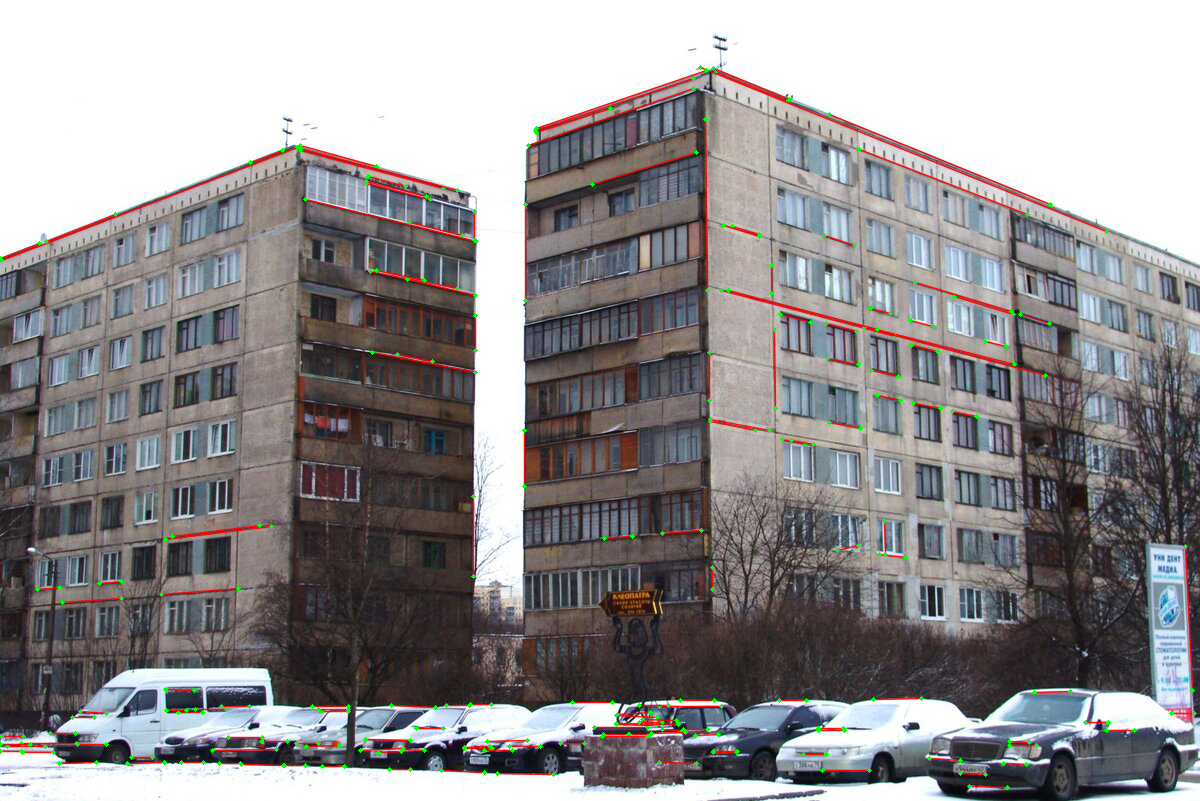
\includegraphics[width=\linewidth]{canny_hl_i2.png}
            \caption{Архитектура\\Максимальная длина линии: 438p\\Минимальная длина линии: 20p\\Всего линий: 160}
            \label{fig:canny_hl_i2}
        \end{subfigure}
        \hfill
        \begin{subfigure}{0.3\textwidth}
            \centering
            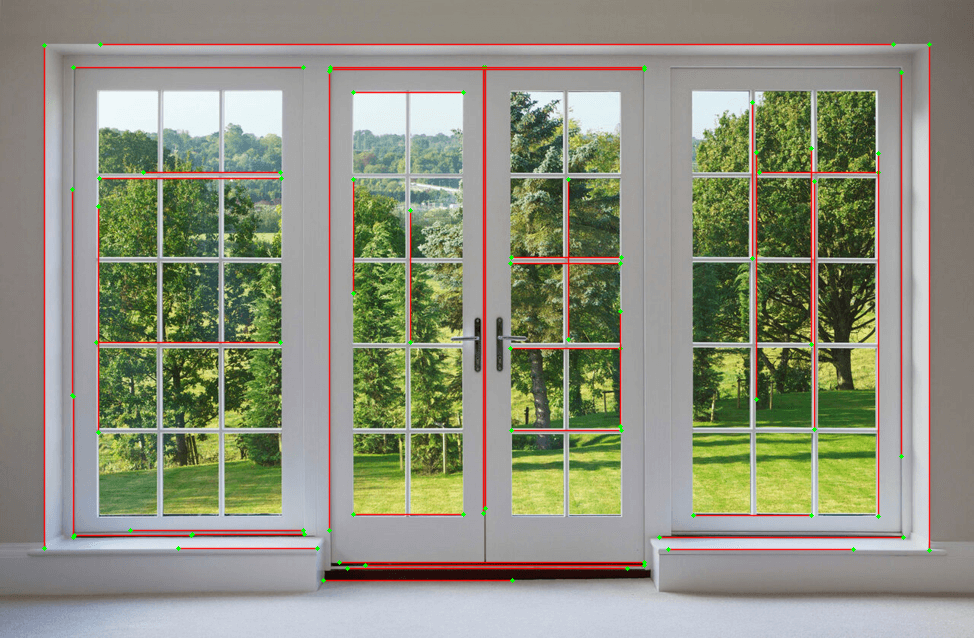
\includegraphics[width=\linewidth]{canny_hl_i3.png}
            \caption{Интерьер\\Максимальная длина линии: 793p\\Минимальная длина линии: 110p\\Всего линий: 43}
            \label{fig:canny_hl_i3}
        \end{subfigure}
        \caption{Алгоритм Хафа на выбранных обработанных изображениях.}
        \label{fig:canny_hl_is}
    \end{figure}


    \noindent Для штрихкода линии были найдены почти идеально -- все вертикальные линии отображены, однако есть погрешности
    в некоторых из них -- линии залезают на числа ниже черных полос. Также появились лишние горизонтальные линии. Для архитектуры
    линии были найдены неплохо, были определены верхние контуры зданий, а также контуры окон, балконов и некоторых полос на самих зданиях.
    Кроме того выделены контуры фар, автомобильных окон, номерных знаков и бамперов. Для интерьера алгоритм Хафа справился хорошо --
    большинство линий в точности повторяют прямоугольные контуры окошек в дверях, какие то выбросы по типу линий <<за окнами>> или
    <<на окнах>> отсутствуют.


    \noindent На рисунке \ref{fig:canny_par_space_is} для каждого исходного изображения отображено пространство признаков преобразования Хафа.
    На оси OX находятся углы в градусах, на OY расстояние в пикселях.
    Исходя из результатов можно сделать вывод, что для штрихкода большинство линий сосредоточено в диапазонах
    $[-100^{\circ},-60^{\circ}]$ и $[60^{\circ},100^{\circ}]$. Для архитектуры линии хорошо просматриваются при примерно
    $-100^{\circ},-80^{\circ},\,80^{\circ},\,100^{\circ}$. Для интерьера больше всего линий сконцентрировано в диапазоне
    $[60^{\circ},100^{\circ}]$.


    \newpage
    \begin{figure}[htbp]
        \centering
        \begin{subfigure}{0.3\textwidth}
            \centering
            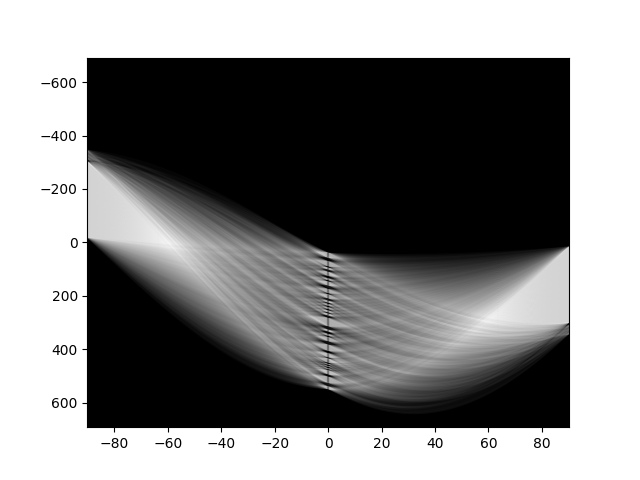
\includegraphics[width=\linewidth]{canny_par_space_i1.png}
            \caption{Штрихкод}
            \label{fig:canny_par_space_i1}
        \end{subfigure}
        \hfill
        \begin{subfigure}{0.3\textwidth}
            \centering
            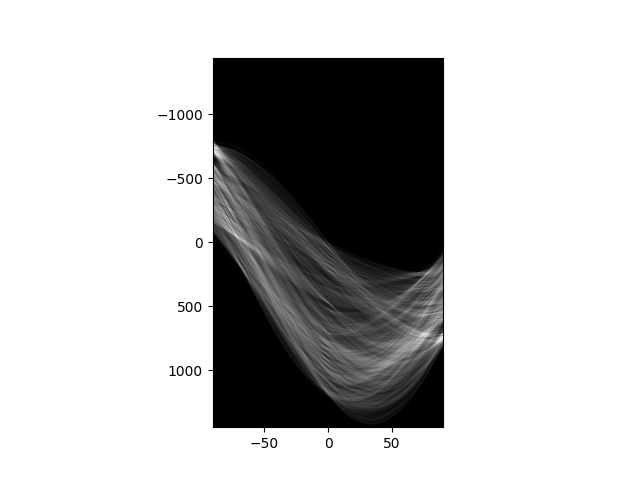
\includegraphics[width=\linewidth]{canny_par_space_i2.png}
            \caption{Архитектура}
            \label{fig:canny_par_space_i2}
        \end{subfigure}
        \hfill
        \begin{subfigure}{0.3\textwidth}
            \centering
            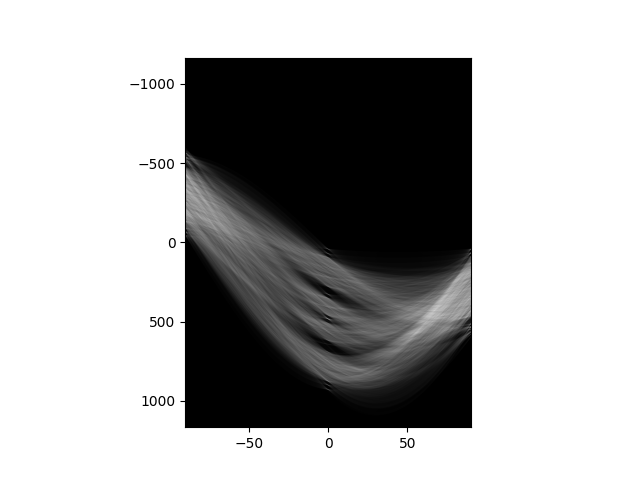
\includegraphics[width=\linewidth]{canny_par_space_i3.png}
            \caption{Интерьер}
            \label{fig:canny_par_space_i3}
        \end{subfigure}
        \caption{Пространство параметров для каждого исходного изображения.}
        \label{fig:canny_par_space_is}
    \end{figure}


    \subsection{Поиск окружностей}
    \noindent Выберем три произвольных изображения, содержащих окружности.
    \begin{figure}[htbp]
        \centering
        \begin{subfigure}{0.3\textwidth}
            \centering
            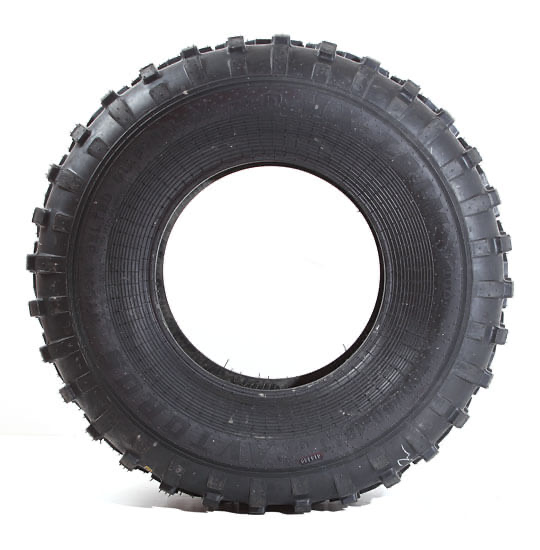
\includegraphics[scale=0.15]{ci1.png}
            \caption{Шина}
            \label{fig:ci1}
        \end{subfigure}
        \hfill
        \begin{subfigure}{0.3\textwidth}
            \centering
            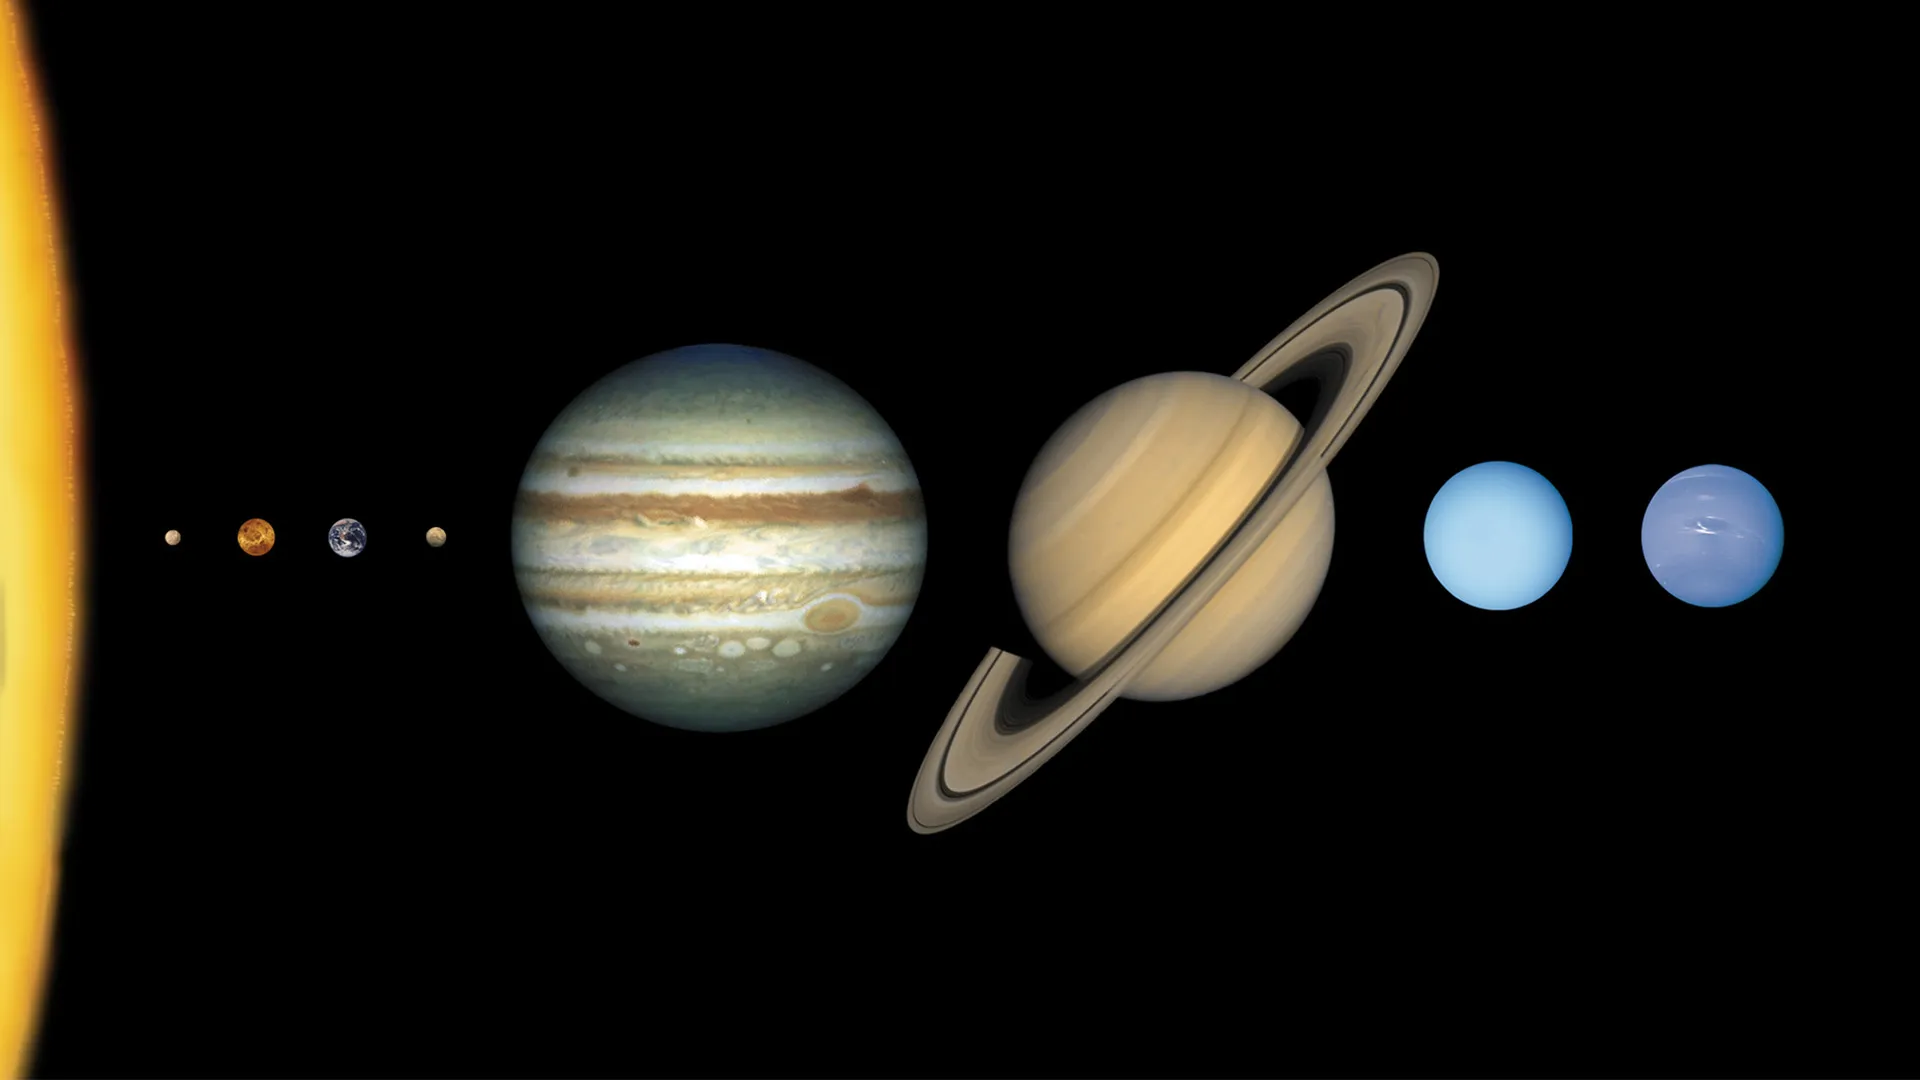
\includegraphics[width=\linewidth]{ci2.png}
            \caption{Солнечная система}
            \label{fig:ci2}
        \end{subfigure}
        \hfill
        \begin{subfigure}{0.3\textwidth}
            \centering
            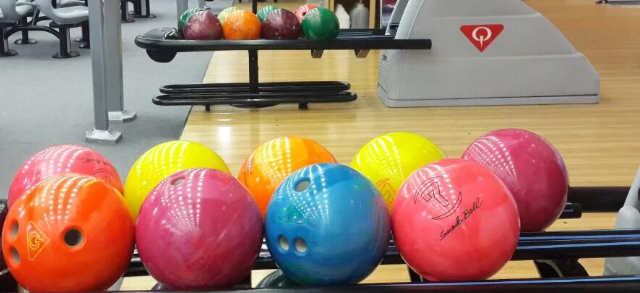
\includegraphics[width=\linewidth]{ci3.png}
            \caption{Шары для боулинга}
            \label{fig:ci3}
        \end{subfigure}
        \caption{Произвольные изображения, содержащие окружности.}
        \label{fig:cis}
    \end{figure}


    \noindent Попробуем сразу применить преобразование Хафа без использования каких-либо дифференциальных операторов.
    Сначала преобразуем изображение к оттенкам серого, далее применим Хафа и нарисуем окружности на оригинальном изображении.
    \begin{figure}[htbp]
        \centering
        \begin{subfigure}{0.3\textwidth}
            \centering
            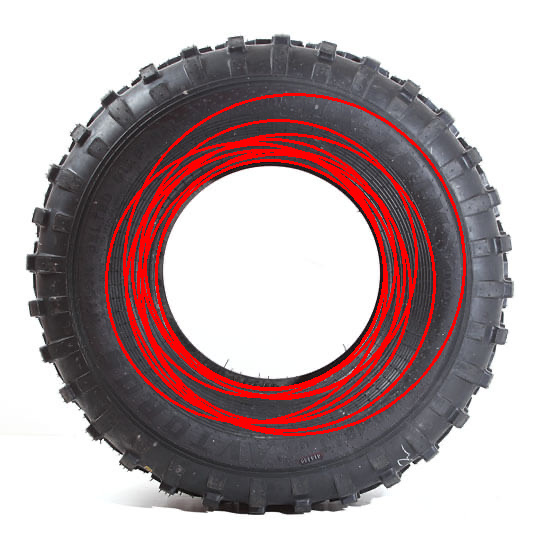
\includegraphics[scale=0.15]{hc_ci1.png}
            \caption{Шина}
            \label{fig:hc_ci1}
        \end{subfigure}
        \hfill
        \begin{subfigure}{0.3\textwidth}
            \centering
            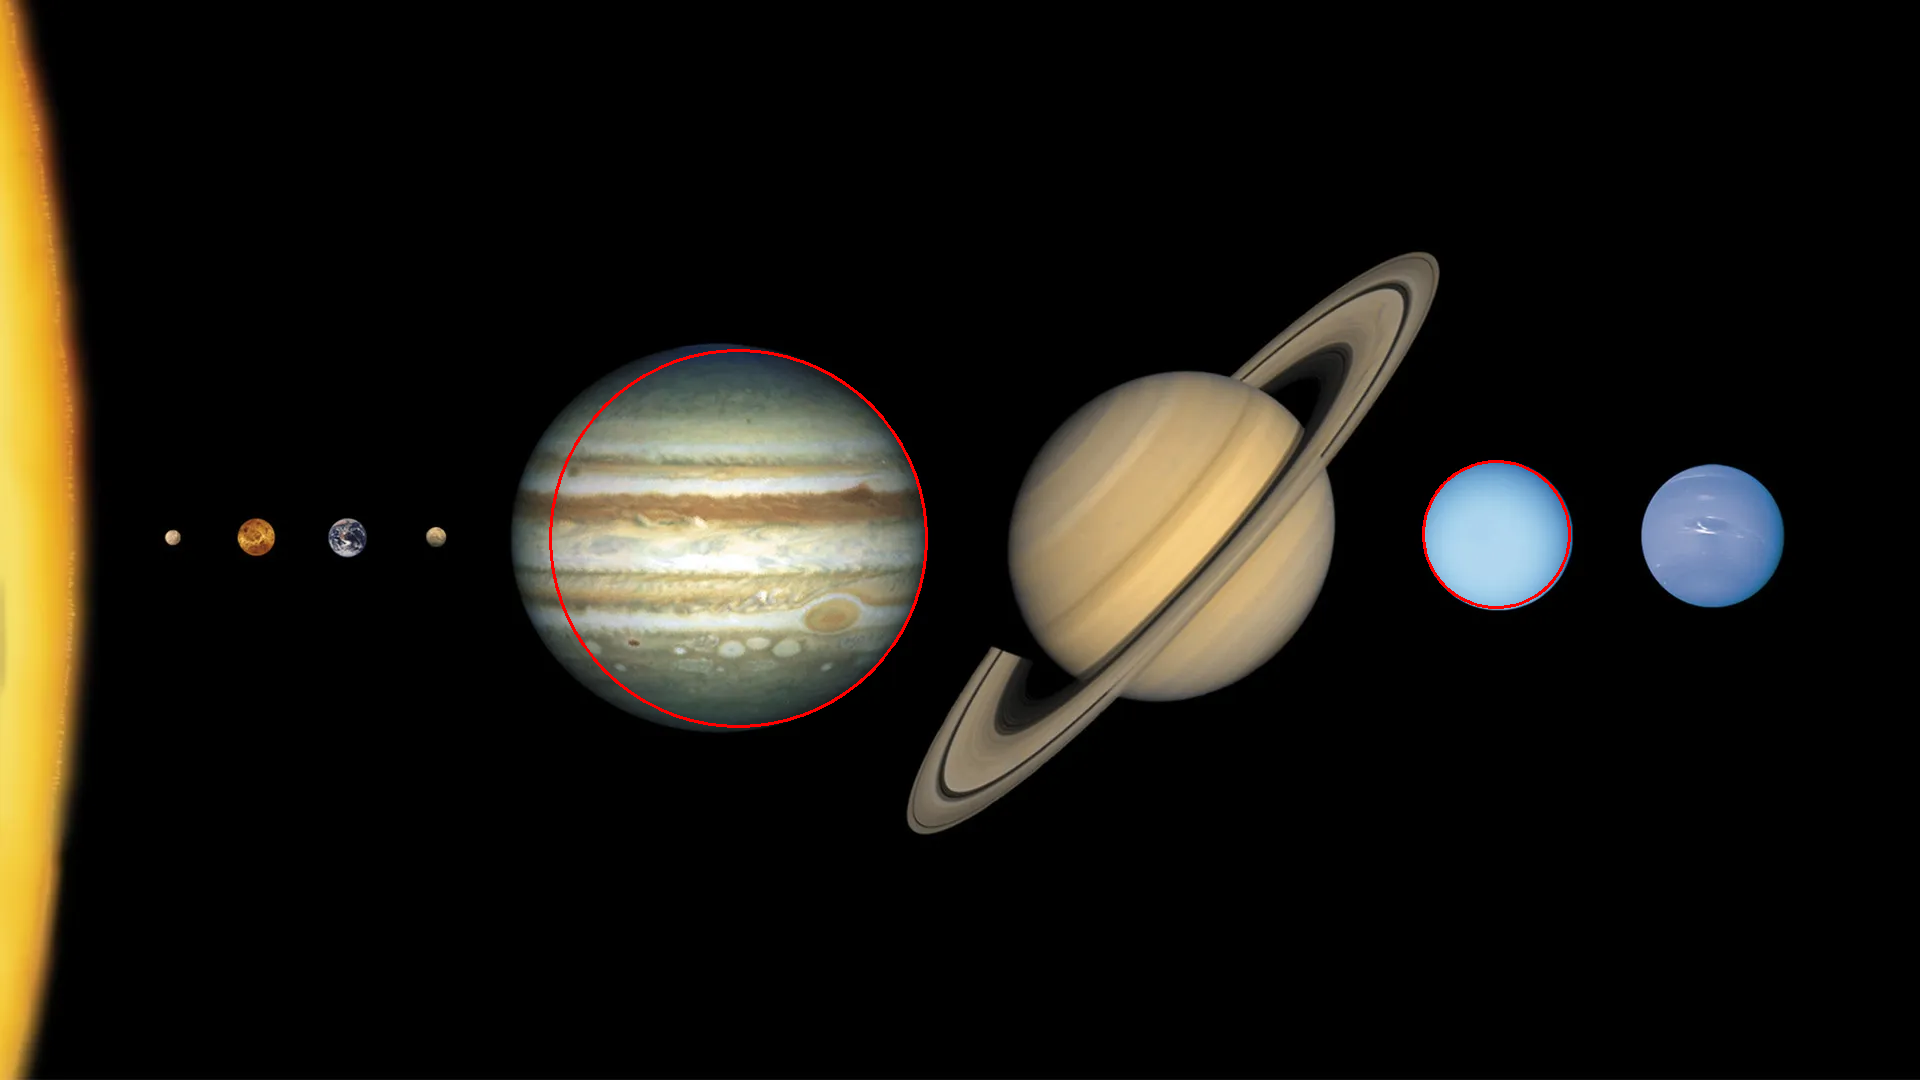
\includegraphics[width=\linewidth]{hc_ci2.png}
            \caption{Солнечная система}
            \label{fig:hc_ci2}
        \end{subfigure}
        \hfill
        \begin{subfigure}{0.3\textwidth}
            \centering
            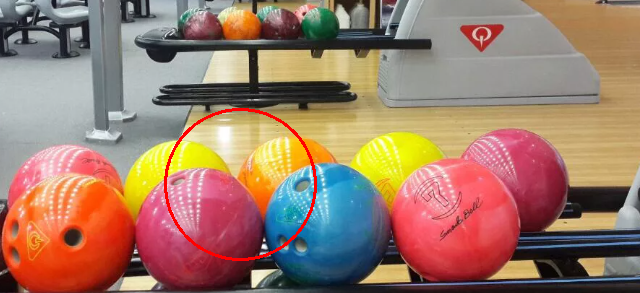
\includegraphics[width=\linewidth]{hc_ci3.png}
            \caption{Шары для боулинга}
            \label{fig:hc_ci3}
        \end{subfigure}
        \caption{Преобразование Хафа на выбранных изображениях.}
        \label{fig:hc_cis}
    \end{figure}


    \noindent Результаты здесь немного лучше, чем результаты поиска линий. Для шины были найдены окружности, которые
    походят на правду, но ничего конкретного не выделяют, хорошо получился только контур отверстия шины, хоть и приближенно.
    В солнечной системе удалось выделить две окружности -- контур Юпитера и Урана. Однако стоит помнить, что планеты в большинстве
    своем представляются эллипсоидами, поэтому получить точный контур того же Юпитера не получится. Для шаров для боулинга результат
    плохой -- не выделен ни один шар, есть какая-то окружность левее середины, не выделяющая никакой контур. Предположительно, неплохие
    результаты для первых двух изображений получились вследствие заметного контраста между объектами, которые нам хотелось бы выделить, и
    фоном, что не сказать про третью картинку.


    \noindent Обработаем изображения алгоритмом Собеля -- дискретным дифференциальный оператором, вычисляющим приближённое значение градиента яркости изображения.
    Оператор основан на свёртке изображения небольшими сепарабельными целочисленными фильтрами в вертикальном и горизонтальном направлениях, поэтому его относительно легко вычислять,
    однако используемая им аппроксимация градиента достаточно грубая. В общем результат обработки очень похож на результат применения алгоритма Кэнни и представлен на рисунке \ref{fig:canny_cis}.


    \newpage
    \begin{figure}[htbp]
        \centering
        \begin{subfigure}{0.3\textwidth}
            \centering
            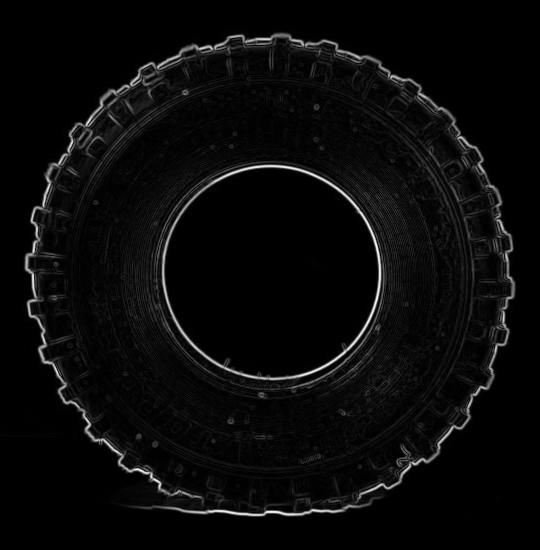
\includegraphics[scale=0.15]{canny_ci1.png}
            \caption{Шина}
            \label{fig:canny_ci1}
        \end{subfigure}
        \hfill
        \begin{subfigure}{0.3\textwidth}
            \centering
            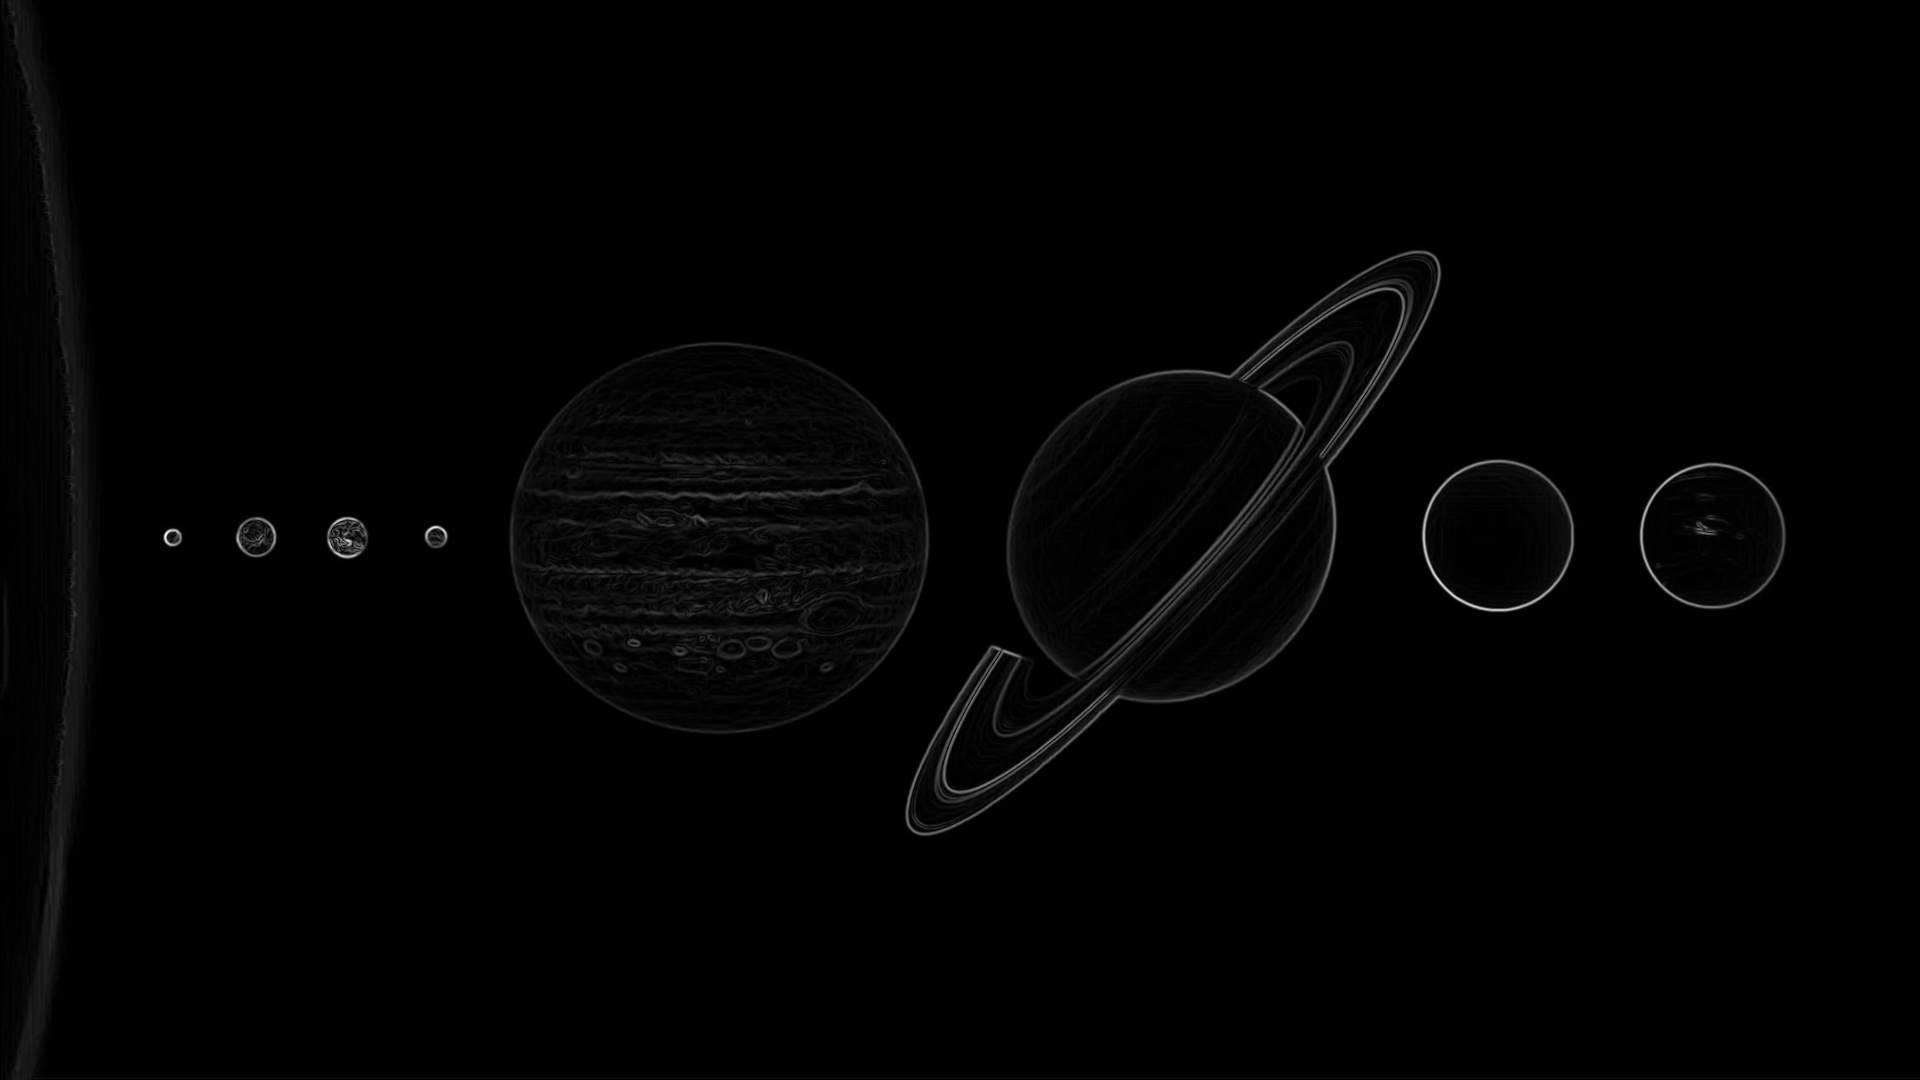
\includegraphics[width=\linewidth]{canny_ci2.png}
            \caption{Солнечная система}
            \label{fig:canny_ci2}
        \end{subfigure}
        \hfill
        \begin{subfigure}{0.3\textwidth}
            \centering
            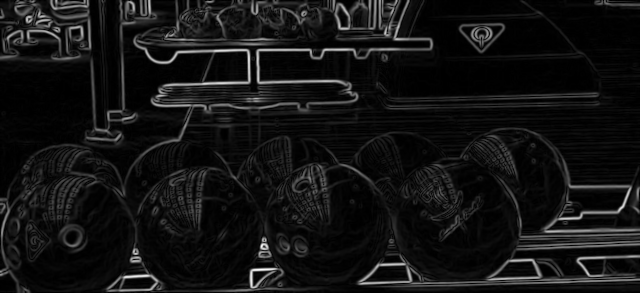
\includegraphics[width=\linewidth]{canny_ci3.png}
            \caption{Шары для боулинга}
            \label{fig:canny_ci3}
        \end{subfigure}
        \caption{Алгоритм Собеля на выбранных изображениях.}
        \label{fig:canny_cis}
    \end{figure}


    \noindent Преобразуем изображения алгоритмом Хафа и получим результат, представленный на рисунке \ref{fig:canny_hc_cis}.
    Найденные окружности отрисованы красным цветом. Ниже каждой картинки написаны радиус в пикселях самой большой и самой маленькой окружностей,
    а также количество отрисованных окружностей.
    \begin{figure}[htbp]
        \centering
        \begin{subfigure}{0.3\textwidth}
            \centering
            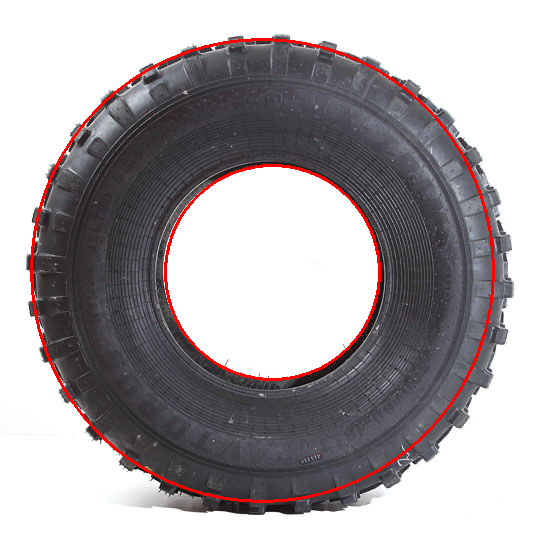
\includegraphics[scale=0.15]{canny_hc_ci1.png}
            \caption{Шина\\Макс. радиус окружности: 231p\\Мин. радиус окружности: 107p\\Всего окружностей: 2}
            \label{fig:canny_hc_ci1}
        \end{subfigure}
        \hfill
        \begin{subfigure}{0.3\textwidth}
            \centering
            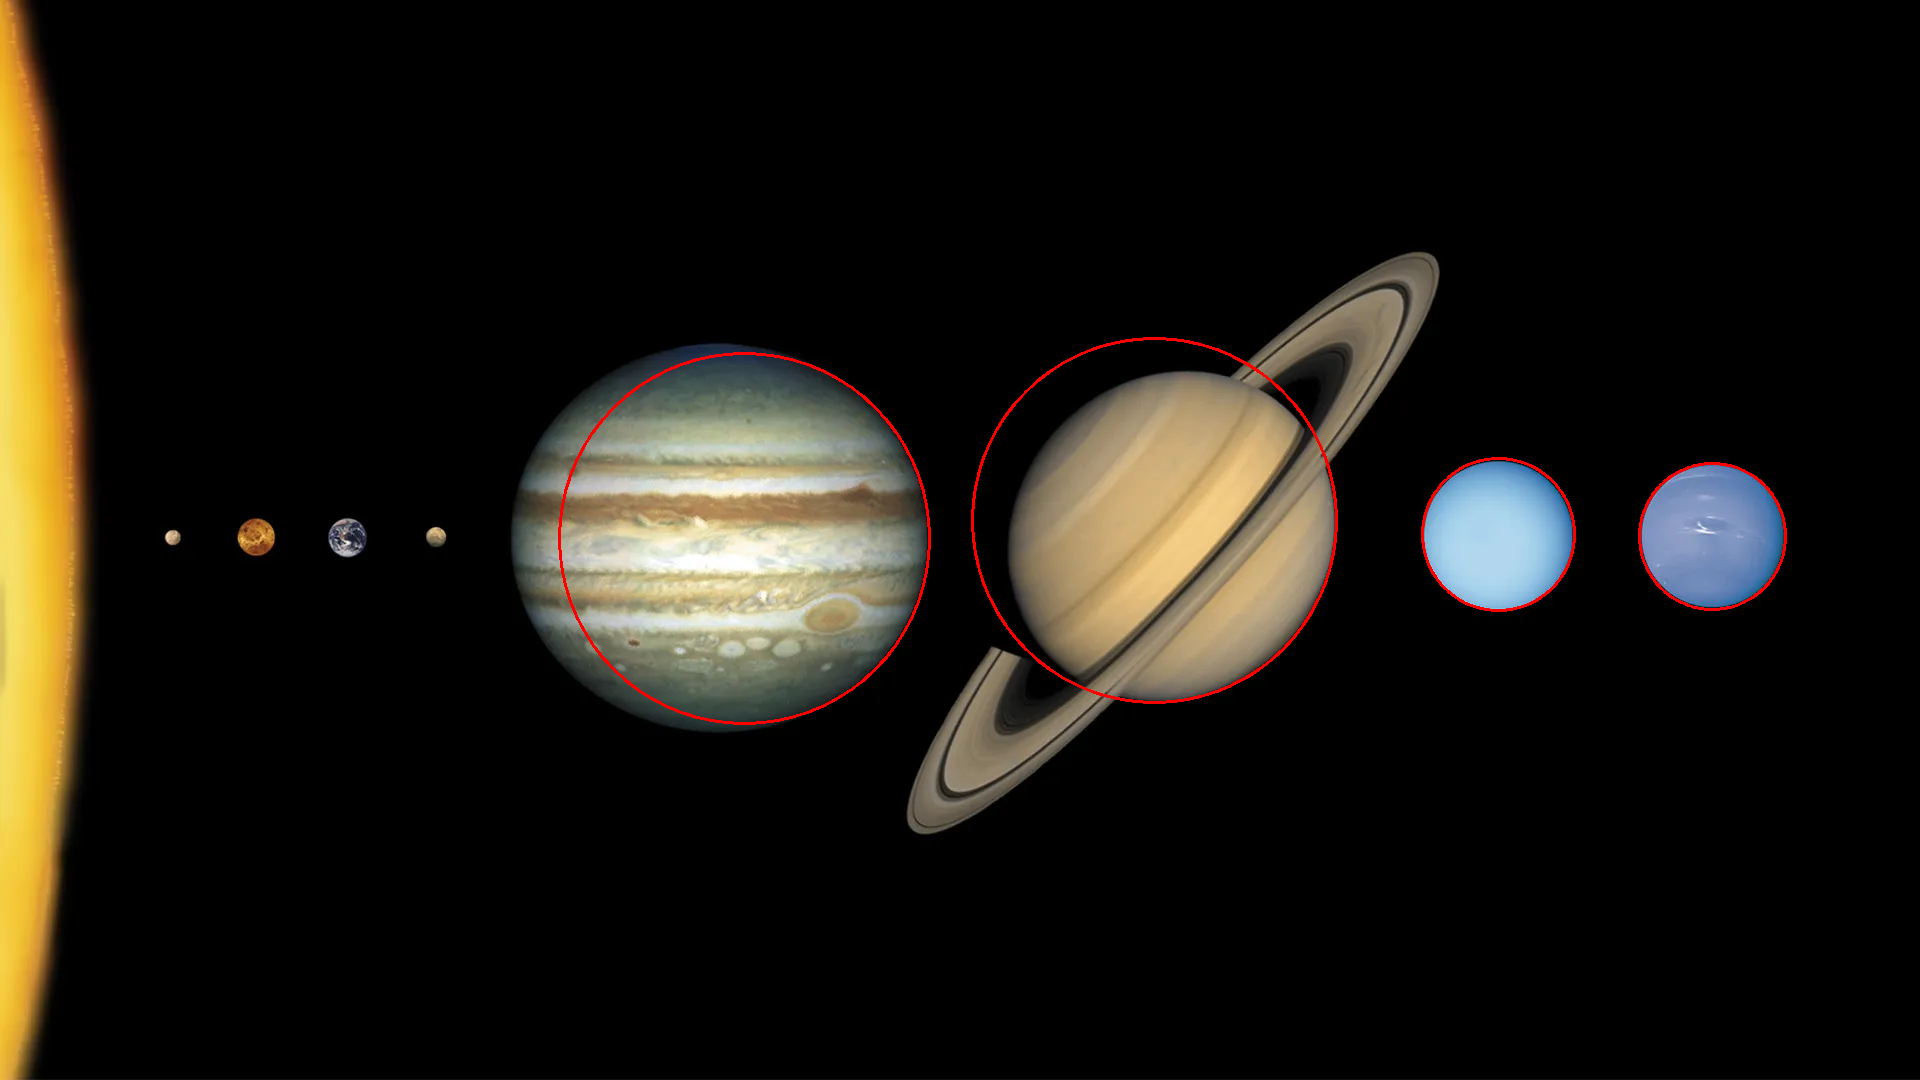
\includegraphics[width=\linewidth]{canny_hc_ci2.png}
            \caption{Солнечная система\\Макс. радиус окружности: 185p\\Мин. радиус окружности: 73p\\Всего окружностей: 4}
            \label{fig:canny_hc_ci2}
        \end{subfigure}
        \hfill
        \begin{subfigure}{0.3\textwidth}
            \centering
            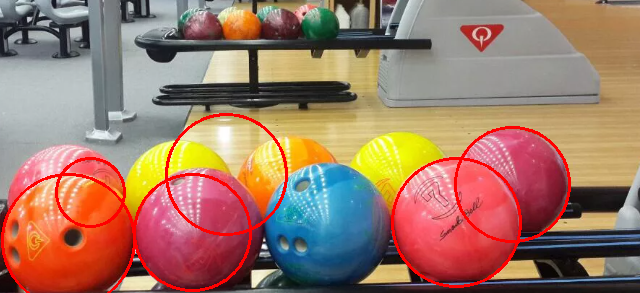
\includegraphics[width=\linewidth]{canny_hc_ci3.png}
            \caption{Шары для боулинга\\Макс. радиус окружности: 66p\\Мин. радиус окружности: 34p\\Всего окружностей: 6}
            \label{fig:canny_hc_ci3}
        \end{subfigure}
        \caption{Алгоритм Хафа на выбранных обработанных изображениях.}
        \label{fig:canny_hc_cis}
    \end{figure}


    \noindent Для шины были найдены две окружности, повторяющие контур отверстия и внешней части, никаких лишних выбросов не обнаружено.
    В солнечной системе стало отрисовано на две планеты больше -- были захвачены Сатурн и Нептун. Для шаров для боулинга отрисовались контуры
    четырех шаров, однако есть две окружности, которые можно назвать выбросами. Причина их появления заключается в не очень хорошей отрисовке контуров
    после применения алгоритма Собеля к исходному изображению -- на рисунке \ref{fig:canny_cis} видно, что на третьем изображении намного лучше выделено
    окружение шаров, чем они сами. Тем не менее алгоритм Хафа достаточно хорошо справился с поиском окружностей.


    \noindent Поиск окружностей радиуса 90 пикселей алгоритмом Хафа для исходных изображений без дифференциальных преобразований представлен на рисунке \ref{fig:hc_r90_cis}.
    \begin{figure}[htbp]
        \centering
        \begin{subfigure}{0.3\textwidth}
            \centering
            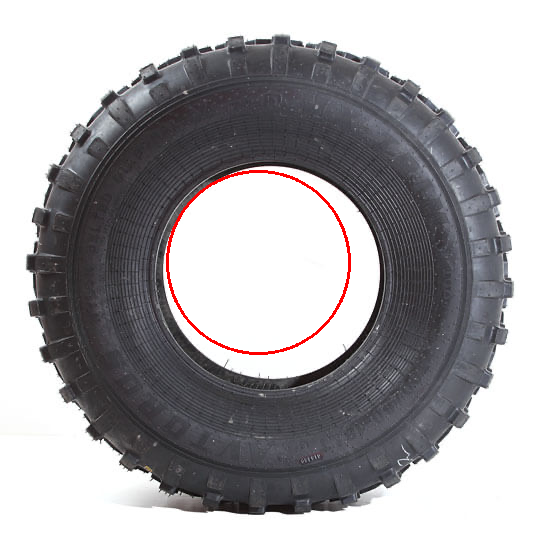
\includegraphics[scale=0.15]{hc_r=90_ci1.png}
            \caption{Шина}
            \label{fig:hc_r90_ci1}
        \end{subfigure}
        \hfill
        \begin{subfigure}{0.3\textwidth}
            \centering
            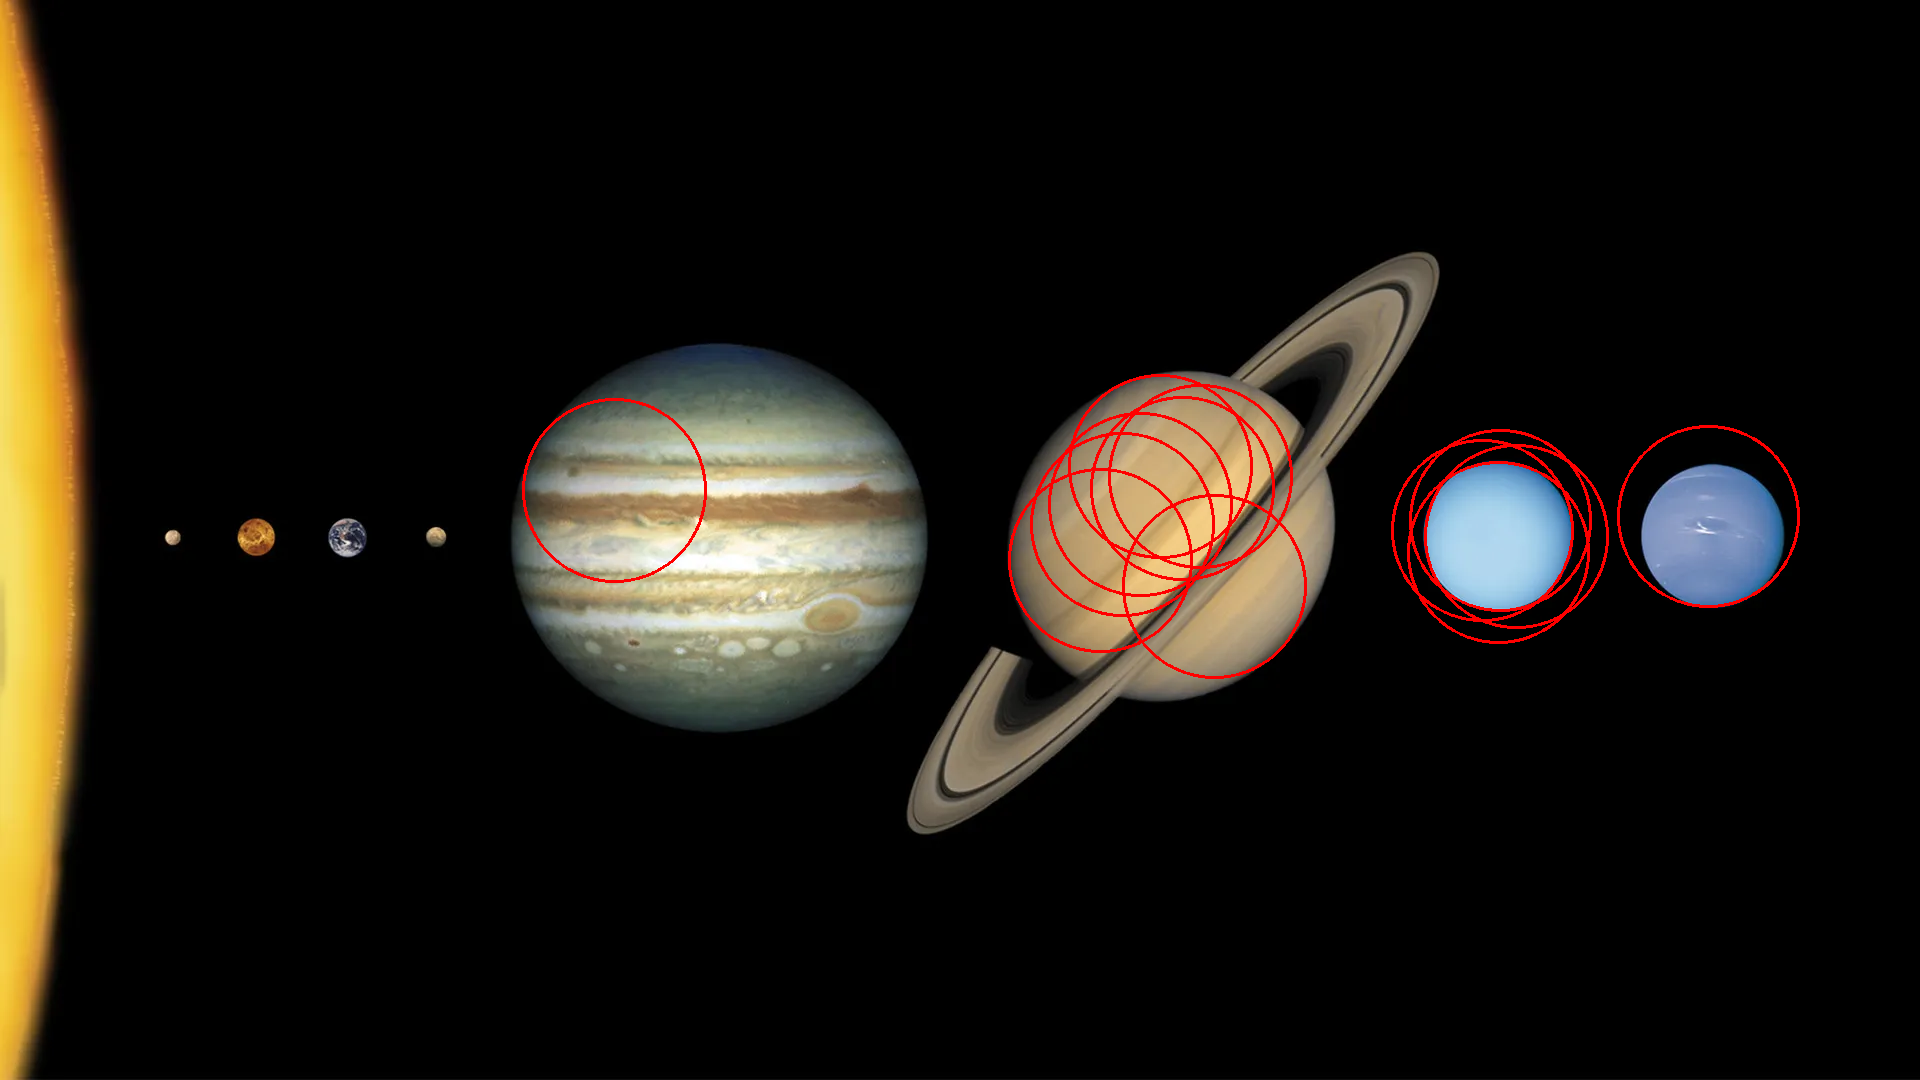
\includegraphics[width=\linewidth]{hc_r=90_ci2.png}
            \caption{Солнечная система}
            \label{fig:hc_r90_ci2}
        \end{subfigure}
        \hfill
        \begin{subfigure}{0.3\textwidth}
            \centering
            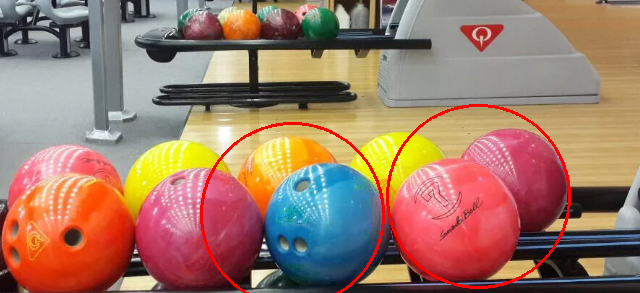
\includegraphics[width=\linewidth]{hc_r=90_ci3.png}
            \caption{Шары для боулинга}
            \label{fig:hc_r90_ci3}
        \end{subfigure}
        \caption{Поиск окружностей радиуса 90 пикселей алгоритмом Хафа на исходных изображениях.}
        \label{fig:hc_r90_cis}
    \end{figure}


    \noindent Как видим, алгоритм отработал верно -- все окружности выглядят одинаково, а значит одного радиуса.


    \noindent Поиск окружностей радиуса 90 пикселей алгоритмом Хафа для исходных изображений с алгоритмом Собеля представлен на рисунке \ref{fig:canny_hc_r90_cis}.
    Алгоритм отработал аналогично, однако окружностей стало больше, за исключением случая с шиной.


    \newpage
    \begin{figure}[htbp]
        \centering
        \begin{subfigure}{0.3\textwidth}
            \centering
            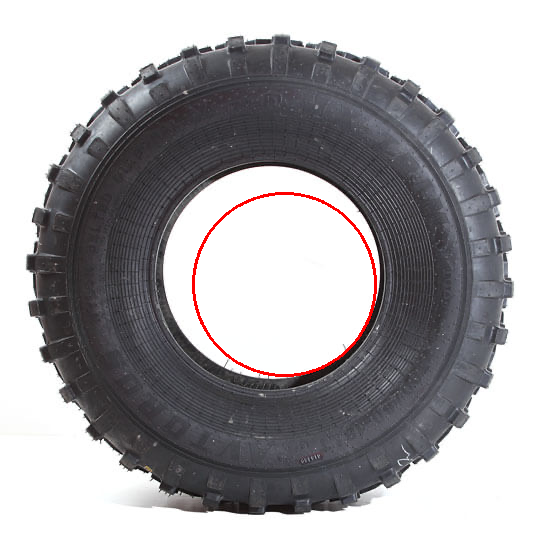
\includegraphics[scale=0.15]{canny_hc_r=90_ci1.png}
            \caption{Шина}
            \label{fig:canny_hc_r90_ci1}
        \end{subfigure}
        \hfill
        \begin{subfigure}{0.3\textwidth}
            \centering
            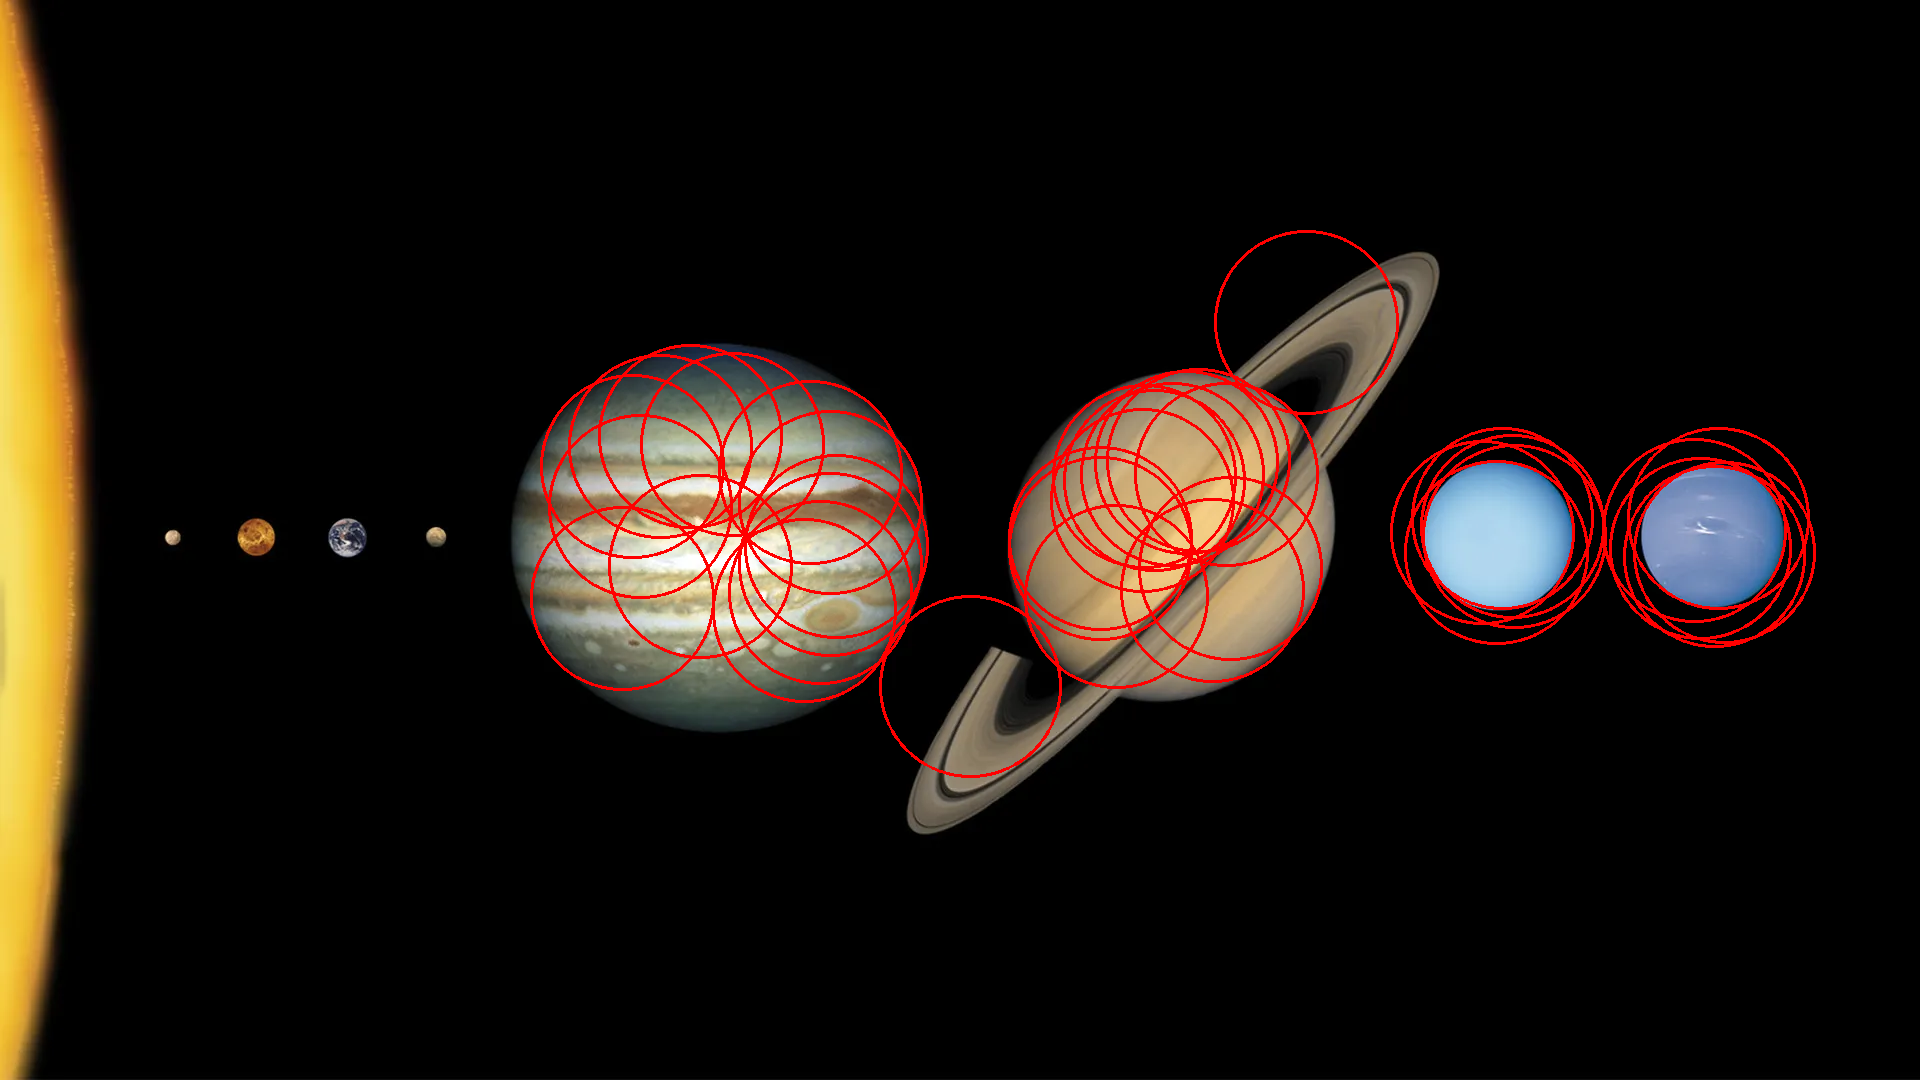
\includegraphics[width=\linewidth]{canny_hc_r=90_ci2.png}
            \caption{Солнечная система}
            \label{fig:canny_hc_r90_ci2}
        \end{subfigure}
        \hfill
        \begin{subfigure}{0.3\textwidth}
            \centering
            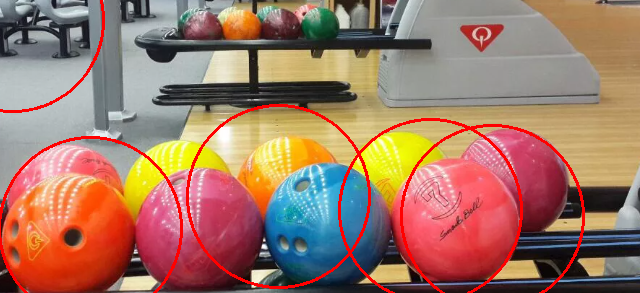
\includegraphics[width=\linewidth]{canny_hc_r=90_ci3.png}
            \caption{Шары для боулинга}
            \label{fig:canny_hc_r90_ci3}
        \end{subfigure}
        \caption{Поиск окружностей радиуса 90 пикселей алгоритмом Хафа на обработанных изображениях.}
        \label{fig:canny_hc_r90_cis}
    \end{figure}


    \subsection{Листинги программных реализаций}
    \noindent Условимся, что кодом ниже мы считываем изображение и преобразуем его к серым тонам всегда при использовании алгоритма Хафа.
    \begin{lstlisting}[label=code0, caption={Считывание изображения и преобразование к серым тонам.}]
    render_to = 'renders'
    src_dir = 'img'
    curr_img = 'ci3.png'
    filename = f'{src_dir}/{curr_img}'
    clr_src = cv2.imread(cv2.samples.findFile(filename), cv2.IMREAD_COLOR)
    src = cv2.cvtColor(clr_src, cv2.COLOR_BGR2GRAY)
    \end{lstlisting}


    \noindent Для начала рассмотрим реализацию алгоритма Хафа для линий. Для поиска линий используется метод detect\_{lines}, в котором
    вызывается HoughLinesP -- вероятностное преобразование Хафа -- с передаваемыми параметрами:
    \begin{center}
    1. \textbf{image} -- Изображение (в бинарном представлении или хотя бы в оттенках серого).\\
    2. \textbf{rho} -- Разрешение параметра $r$ в пикселях.\\
    3. \textbf{theta} -- Разрешение параметра $\theta$ в радианах.\\
    4. \textbf{threshold} -- Минимальное количество пересечений для <<обнаружения>> линии.\\
    5. \textbf{minLineLength} -- Минимальное количество точек, которые могут образовывать линию.\\
    6. \textbf{maxLineGap} -- Максимальный разрыв между двумя точками, которые считаются на одной линии.
    \end{center}


    \noindent Метод draw\_{lines} в цикле бегает по линиям и отрисовывает их на переданном в метод изображении по
    координатам начала и конца линии. Также метод отрисовывает точки.
    \begin{lstlisting}[label=code1, caption={Алгоритм Хафа для поиска линий и отрисовки их на изображении.}]
    def detect_lines(src, rho, theta, threshold, minLineLength, maxLineGap):
        lines = cv2.HoughLinesP(
        image=src,
        rho=rho,
        theta=theta,
        threshold=threshold,
        lines=None,
        minLineLength=minLineLength,
        maxLineGap=maxLineGap
    )
    return lines

    def draw_lines(src, lines, thickness=1, color=(0, 0, 255),
                   marker_radius=2, dot_color1=(0, 255, 0), dot_color2=(0, 255, 0)):
        if lines is not None:
            for i in range(0, len(lines)):
                l = lines[i][0]
                x_1, y_1, x_2, y_2 = l[0], l[1], l[2], l[3]
                cv2.line(src, (x_1, y_1), (x_2, y_2), color, thickness, cv2.LINE_AA)
                cv2.circle(src, (x_1, y_1), marker_radius, dot_color1, -1)
                cv2.circle(src, (x_2, y_2), marker_radius, dot_color2, -1)

    return src
    \end{lstlisting}


    \noindent Для отрисовывания пространства параметров использовался код, представленный на листинге \ref{code2}.
    \begin{lstlisting}[label=code2, caption={Программа для отрисовки пространства параметров для линий.}]
    def parameters_space_lines(src, arr_ang_step=0.1, brightness=3):
        dots = int(round(360 / arr_ang_step))
        angles = np.linspace(-np.pi / 2, np.pi / 2, dots, endpoint=False)
        H, theta, rho = skimage.transform.hough_line(src, theta=angles)

        ang_step = 0.5 * np.diff(theta).mean()
        dis_step = 0.5 * np.diff(rho).mean()

        bounds = [np.rad2deg(theta[0] - ang_step),
                  np.rad2deg(theta[-1] + ang_step),
                  rho[-1] + dis_step, rho[0] - dis_step]
        parameters_space = cv2.cvtColor(np.float32(brightness * H / np.max(H)),
                                        cv2.COLOR_GRAY2RGB)
        return parameters_space, bounds
    \end{lstlisting}


    \noindent Для поиска максимальной и минимальной длины линии был написан код представленный на листинге \ref{code3}.
    \begin{lstlisting}[label=code3, caption={Поиск максимальной и минимальной длины линии.}]
    def min_max_len_lines(lines):
        min_len = float('inf')
        max_len = 0
        min_len_line = None
        max_len_line = None

        if lines is not None:
            for line in lines:
                x1, y1, x2, y2 = line[0]

                line_len = ((x2 - x1) ** 2 + (y2 - y1) ** 2) ** 0.5
                if line_len > max_len:
                    max_len = line_len
                    max_len_line = line
                if line_len < min_len:
                    min_len = line_len
                    min_len_line = line

        return min_len, min_len_line, max_len, max_len_line
    \end{lstlisting}


    \noindent Пример использования кода с предыдущих листингов расположен на листинге \ref{code4}.
    \begin{lstlisting}[label=code4, caption={Пример использования программы для поиска линий и построения пространства параметров.}]
    rho = 1
    theta = np.pi / 180
    threshold = 130
    threshold1 = 350
    threshold2 = 230
    apertureSize = 3
    minLineLength = 20
    maxLineGap = 5

    edge_src = cv2.Canny(src, threshold1, threshold2, None, apertureSize)
    lines_edge_src = detect_lines(edge_src, rho, theta,
                                  threshold, minLineLength, maxLineGap)
    output_edge_src = draw_lines(clr_src.copy(), lines_edge_src)
    ps_pace, bds = parameters_space_lines(edge_src)

    edge_min_len, edge_min_len_l, edge_max_len, edge_max_len_l = min_max_len_lines(lines_edge_src)
    edge_lines_count = len(lines_edge_src)

    cv2.imwrite(f'{render_to}/canny_{curr_img}', edge_src)
    plt.imshow(ps_pace, extent=bds, aspect=0.1)
    plt.savefig(f'{render_to}/canny_par_space_{curr_img}')
    cv2.imwrite(f'{render_to}/canny_hl_{curr_img}', output_edge_src)
    print(f'canny_max_len_line={edge_max_len}p\ncanny_min_len_line={edge_min_len}p\n'
          f'canny_lines_count={edge_lines_count}')
    \end{lstlisting}


    \noindent Для окружностей реализация почти такая же, но пропадают и добавляются некоторые параметры:
    \begin{center}
        1. \textbf{method} -- Метод преобразования Хафа <<Градиент>>, который используется для обнаружения окружностей.\\
        2. \textbf{dp} -- Параметр, который определяет коэффициент разреженности аккумуляторной матрицы преобразования Хафа.\\
        3. \textbf{minDist} -- Минимальное расстояние между центрами обнаруженных окружностей.\\
        4. \textbf{param1} -- Параметр для определения порогового значения для детекции границ окружностей на изображении.\\
        5. \textbf{param2} -- Параметр для определения минимального числа голосов, которые должна получить окружность, чтобы она была признана окружностью.\\
        6. \textbf{minRadius} -- Минимальный радиус ожидаемой окружности.\\
        7. \textbf{maxRadius} -- Максимальный радиус ожидаемой окружности.\\
    \end{center}


    \noindent Метод draw\_{circles} бегает по окружностям и рисует их на передаваемом изображении с помощью
    координат центра окружности i[0], i[1] и радиуса окружности i[2].
    \begin{lstlisting}[label=code5, caption={Алгоритм Хафа для поиска и отрисовки окружностей.}]
    def detect_circles(src, dp, min_dis, par1, par2, min_r, max_r):
        circles = cv2.HoughCircles(
            image=src,
            method=cv2.HOUGH_GRADIENT,
            dp=dp,
            minDist=min_dis,
            param1=par1,
            param2=par2,
            minRadius=min_r,
            maxRadius=max_r
        )
        return circles
    
    def draw_circles(src, circs, color=(0, 0, 255), thickness=2):
        if circs is not None:
            circles = np.uint16(np.around(circs))
            for i in circles[0, :]:
                cv2.circle(src, (i[0], i[1]), i[2], color, thickness)
        return src
    \end{lstlisting}


    \noindent Также написан метод для поиска минимального и максимального радиусов найденных окружностей.
    \begin{lstlisting}[label=code6, caption={Поиск минимального и максимального радиуса найденных окружностей.}]
    def min_max_radius_circles(circles):
        min_radius = float('inf')
        max_radius = 0
        min_circle = None
        max_circle = None
    
        if circles is not None:
            circles = np.uint16(np.around(circles))
            for i in circles[0, :]:
                if i[2] < min_radius:
                    min_radius = i[2]
                    min_circle = i
                if i[2] > max_radius:
                    max_radius = i[2]
                    max_circle = i
    
        return min_radius, min_circle, max_radius, max_circle
    \end{lstlisting}


    \noindent Пример использования методов, описанных в предыдущих листингах, расположен на листинге \ref{code7}.
    \begin{lstlisting}[label=code7, caption={Пример применения алгоритма Хафа для поиска окружностей.}]
    sobelx = cv2.Sobel(src, cv2.CV_64F, 1, 0, ksize=5)
    sobely = cv2.Sobel(src, cv2.CV_64F, 0, 1, ksize=5)
    edge_src = np.hypot(sobelx, sobely)
    edge_src = np.uint8(edge_src / np.max(edge_src) * 255)

    dp = 1
    min_dis = 10
    par1 = 40
    par2 = 10
    min_r = 30
    max_r = 95
    single_r = 90

    circles_edge_src = detect_circles(edge_src, dp, min_dis, par1, par2, min_r, max_r)
    output_edge_src = draw_circles(clr_src.copy(), circles_edge_src)

    edge_min_radius, edge_min_circle, edge_max_radius, edge_max_circle = min_max_radius_circles(circles_edge_src)
    edge_circs_count = len(circles_edge_src[0])

    circles_edge_src2 = detect_circles(edge_src, dp, min_dis, par1, par2, single_r, single_r)
    output_edge_src2 = draw_circles(clr_src.copy(), circles_edge_src2)

    cv2.imwrite(f'{render_to}/canny_{curr_img}', edge_src)
    cv2.imwrite(f'{render_to}/canny_hc_{curr_img}', output_edge_src)
    cv2.imwrite(f'{render_to}/canny_hc_r={single_r}_{curr_img}', output_edge_src2)
    print(f'min_radius={edge_min_radius}p\nmax_radius={edge_max_radius}p\ncircles_count={edge_circs_count}\n')
    \end{lstlisting}


    \subsection{Дополнительные сведения}
    \noindent Для штрихкода использовались следующие параметры:
    \begin{center}
        1. \textbf{image=src}\\
        2. \textbf{rho=1}\\
        3. \textbf{theta=np.pi / 180}\\
        4. \textbf{threshold=50}\\
        5. \textbf{threshold1=50}\\
        6. \textbf{threshold2=200}\\
        7. \textbf{apertureSize=3}\\
        8. \textbf{minLineLength=50}\\
        9. \textbf{maxLineGap=10}
    \end{center}


    \noindent Для архитектуры использовались следующие параметры:
    \begin{center}
        1. \textbf{image=src}\\
        2. \textbf{rho=1}\\
        3. \textbf{theta=np.pi / 180}\\
        4. \textbf{threshold=130}\\
        5. \textbf{threshold1=350}\\
        6. \textbf{threshold2=230}\\
        7. \textbf{apertureSize=3}\\
        8. \textbf{minLineLength=20}\\
        9. \textbf{maxLineGap=5}
    \end{center}


    \noindent Для интерьера использовались следующие параметры:
    \begin{center}
        1. \textbf{image=src}\\
        2. \textbf{rho=1}\\
        3. \textbf{theta=np.pi / 180}\\
        4. \textbf{threshold=150}\\
        5. \textbf{threshold1=300}\\
        6. \textbf{threshold2=110}\\
        7. \textbf{apertureSize=3}\\
        8. \textbf{minLineLength=110}\\
        9. \textbf{maxLineGap=5}
    \end{center}


    \noindent Для шины использовались следующие параметры:
    \begin{center}
        1. \textbf{dp=1}\\
        2. \textbf{minDist=10}\\
        3. \textbf{param1=100}\\
        4. \textbf{param2=250}\\
        5. \textbf{minRadius=30}\\
        6. \textbf{maxRadius=250}
    \end{center}


    \noindent Для солнечной системы использовались следующие параметры:
    \begin{center}
        1. \textbf{dp=1}\\
        2. \textbf{minDist=180}\\
        3. \textbf{param1=50}\\
        4. \textbf{param2=100}\\
        5. \textbf{minRadius=10}\\
        6. \textbf{maxRadius=300}
    \end{center}

    
    \noindent Для шины использовались следующие параметры:
    \begin{center}
        1. \textbf{dp=1}\\
        2. \textbf{minDist=55}\\
        3. \textbf{param1=100}\\
        4. \textbf{param2=50}\\
        5. \textbf{minRadius=30}\\
        6. \textbf{maxRadius=95}
    \end{center}


    \section{Ответы на вопросы}
    \subsection{Какая идея лежит в основе преобразования Хафа?}
    \noindent Идея преобразования Хафа заключается в преобразовании точек изображения
    в параметрическое пространство, где каждая фигура представлена уникальным набором параметров.
    Путем подсчета голосов (аккумуляции) определяются пики в пространстве параметров, которые соответствуют
    возможным фигурам на изображении, позволяя обнаруживать линии, окружности и другие геометрические формы.


    \subsection{Можно ли использовать преобразование Хафа для поиска
    произвольных контуров, которые невозможно описать аналитически?}
    \noindent Преобразование Хафа может быть использовано для поиска произвольных контуров,
    которые невозможно описать аналитически. Это достигается путем создания соответствующего пространства параметров
    из угловых координат и/или радиусов, которые представляют форму необходимого контура. Затем применяется подсчет
    голосов для каждой возможной формы в этом пространстве, позволяя выявить пики, которые соответствуют контурам на изображении.


    \subsection{Что такое рекуррентное и обобщенное преобразования Хафа?}
    \noindent Рекуррентное преобразование Хафа -- одификация преобразования Хафа,
    которая позволяет эффективно работать с более сложными формами, такими как кривые или произвольные формы.
    В отличие от классического преобразования Хафа, которое обрабатывает только фиксированные формы
    (например, прямые линии и окружности), рекуррентное преобразование Хафа использует итеративный процесс
    для поиска более сложных форм путем комбинирования простых форм. 


    \noindent Обобщенное преобразование Хафа -- расширение преобразования Хафа, которое позволяет обнаруживать
    произвольные формы без заранее определенных параметрических уравнений. Вместо этого, GHT представляет каждую
    точку на изображении как объект, который может быть частью произвольной формы. Затем алгоритм просматривает
    все возможные комбинации точек, чтобы найти соответствующие формы. GHT более гибок и может использоваться
    для обнаружения различных форм, включая те, которые сложно описать с помощью аналитических уравнений.


    \subsection{Какие бывают способы параметризации в преобразовании Хафа?}
    \noindent В лабораторной работе были рассмотрены способы параметризации только для линий и окружностей.
    В общем бывают следующие виды параметризации:
    \begin{center}
        \textbf{Для прямых линий:}\\
        1. Угловая и дистанционная (угловая координата и расстояние до начала координат).\\
        2. Угловая и смещение (угловая координата и смещение относительно оси координат).\\
        \textbf{Для окружностей:}\\
        1. Координаты центра и радиус окружности.\\
        \textbf{Для эллипсов:}\\
        1. Координаты центра, большая и малая полуоси, угол наклона эллипса.\\
        \textbf{Для общих кривых:}\\
        1. Параметризация Безье, используемая для описания кривых Безье.\\
        2. Параметризация Б-сплайнов, которая позволяет описывать более сложные кривые.\\
        \textbf{Для произвольных форм:}\\
        1. В обобщенном преобразовании Хафа (GHT) каждая точка изображения рассматривается как параметр,
        и произвольные формы определяются с использованием комбинации этих точек.
    \end{center}

    \section{Выводы о проделанной работе}
    \noindent В ходе данной лабораторной работы были рассмотрены преобразования Хафа для поиска прямых линий и
    окружностей на изображении. Было выяснено, что перед применением алгоритма Хафа необходимо подготовить изображение --
    как минимум сделать в оттенках серого и дифференциальным оператором выделить контуры. В ином случае нет гарантии, что
    алгоритм сработает как нужно -- все зависит от конкретного изображения. Кроме того, вследствие высокой ресурсоемкости
    алгоритма изображение лучше сжать для дальнейшего исследования, иначе будет потрачено много времени, а результат может
    оказаться не подходящим.

\end{document}